 \documentclass[12pt]{article}

%------------- fonts ------------------------------

%\usepackage[T1]{fontenc} % Use 8-bit encoding that has 256 glyphs
%\usepackage{fourier} % Use the Adobe Utopia font for the document - comment this line to return to the LaTeX default
%\usepackage{mathptmx}
%\usepackage{kpfonts}
%\usepackage{stix}
%\usepackage{libertine}
\usepackage[english]{babel} % English language/hyphenation
\usepackage[compact]{titlesec}
\usepackage[bottom]{footmisc} % typesetting of footnotes



%-------------- Math packges ----------------------
\usepackage{amsmath, amssymb, bm, bbm, natbib, babel, units}
%%This is the file ee.sty.
%%This style file underlies the paper
%%"Notation in Econometrics: a proposal for a standard"
%%by Karim Abadir and Jan R. Magnus,
%%The Econometrics Journal (2002), 5, 76-90.
%%
%In order to use the new commands in the
%file ee.sty, the packages amsmath, amssymb,
%and bm should be available. Thus, a paper could
%have the following format:
%
%\documentclass[11pt,dvips,a4paper]{article}
%\usepackage{amsmath}
%\usepackage{amssymb}
%\usepackage{bm}
%%%This is the file ee.sty.
%%This style file underlies the paper
%%"Notation in Econometrics: a proposal for a standard"
%%by Karim Abadir and Jan R. Magnus,
%%The Econometrics Journal (2002), 5, 76-90.
%%
%In order to use the new commands in the
%file ee.sty, the packages amsmath, amssymb,
%and bm should be available. Thus, a paper could
%have the following format:
%
%\documentclass[11pt,dvips,a4paper]{article}
%\usepackage{amsmath}
%\usepackage{amssymb}
%\usepackage{bm}
%%%This is the file ee.sty.
%%This style file underlies the paper
%%"Notation in Econometrics: a proposal for a standard"
%%by Karim Abadir and Jan R. Magnus,
%%The Econometrics Journal (2002), 5, 76-90.
%%
%In order to use the new commands in the
%file ee.sty, the packages amsmath, amssymb,
%and bm should be available. Thus, a paper could
%have the following format:
%
%\documentclass[11pt,dvips,a4paper]{article}
%\usepackage{amsmath}
%\usepackage{amssymb}
%\usepackage{bm}
%\input{ee.sty}
%\begin{document}
%...document text here...
%\end{document}
%
%Alternatively, copy the new commands below and paste them to replace \input{ee.sty}
%in the example above. This second method is the one we have used in the file notation.tex.
%
%%%%%%%%%%%%%%%%%%%%%%%%%%%%%%%
%
\newcommand{\newoperator}[3]{\newcommand*{#1}{\mathop{#2}#3}}
\newcommand{\renewoperator}[3]{\renewcommand*{#1}{\mathop{#2}#3}}
%
% symbols C,N,Q,R,Z for sets
\newcommand{\SC}{\mathbb{C}}
\newcommand{\SN}{\mathbb{N}}
\newcommand{\SQ}{\mathbb{Q}}
\newcommand{\SR}{\mathbb{R}}
\newcommand{\SZ}{\mathbb{Z}}
%
% calligraphic capital letters
\newcommand{\calA}{\mathcal{A}}
\newcommand{\calB}{\mathcal{B}}
\newcommand{\calC}{\mathcal{C}}
\newcommand{\calD}{\mathcal{D}}
\newcommand{\calE}{\mathcal{E}}
\newcommand{\calF}{\mathcal{F}}
\newcommand{\calG}{\mathcal{G}}
\newcommand{\calH}{\mathcal{H}}
\newcommand{\calI}{\mathcal{I}}
\newcommand{\calJ}{\mathcal{J}}
\newcommand{\calK}{\mathcal{K}}
\newcommand{\calL}{\mathcal{L}}
\newcommand{\calM}{\mathcal{M}}
\newcommand{\calN}{\mathcal{N}}
\newcommand{\calO}{\mathcal{O}}
\newcommand{\calP}{\mathcal{P}}
\newcommand{\calQ}{\mathcal{Q}}
\newcommand{\calR}{\mathcal{R}}
\newcommand{\calS}{\mathcal{S}}
\newcommand{\calT}{\mathcal{T}}
\newcommand{\calU}{\mathcal{U}}
\newcommand{\calV}{\mathcal{V}}
\newcommand{\calW}{\mathcal{W}}
\newcommand{\calX}{\mathcal{X}}
\newcommand{\calY}{\mathcal{Y}}
\newcommand{\calZ}{\mathcal{Z}}
%
% bold lowercase and capital letters for vectors (v) and matrices (m)
\newcommand{\mA}{\mathbf A}
\newcommand{\va}{\mathbf a}
\newcommand{\mB}{\mathbf B}
\newcommand{\vb}{\mathbf b}
\newcommand{\mC}{\mathbf C}
\newcommand{\vc}{\mathbf c}
\newcommand{\mD}{\mathbf D}
\newcommand{\vd}{\mathbf d}
\newcommand{\mE}{\mathbf E}
\newcommand{\ve}{\mathbf e}
\newcommand{\mF}{\mathbf F}
\newcommand{\vf}{\mathbf f}
\newcommand{\mG}{\mathbf G}
\newcommand{\vg}{\mathbf g}
\newcommand{\mH}{\mathbf H}
\newcommand{\vh}{\mathbf h}
\newcommand{\mI}{\mathbf I}
\newcommand{\vi}{\mathbf i}
\newcommand{\mJ}{\mathbf J}
\newcommand{\vj}{\mathbf j}
\newcommand{\mK}{\mathbf K}
\newcommand{\vk}{\mathbf k}
\newcommand{\mL}{\mathbf L}
\newcommand{\vl}{\mathbf l}
\newcommand{\mM}{\mathbf M}
\newcommand{\vm}{\mathbf m}
\newcommand{\mN}{\mathbf N}
\newcommand{\vn}{\mathbf n}
\newcommand{\mO}{\mathbf O}
\newcommand{\vo}{\mathbf o}
\newcommand{\mP}{\mathbf P}
\newcommand{\vp}{\mathbf p}
\newcommand{\mQ}{\mathbf Q}
\newcommand{\vq}{\mathbf q}
\newcommand{\mR}{\mathbf R}
\newcommand{\vr}{\mathbf r}
\newcommand{\mS}{\mathbf S}
\newcommand{\vs}{\mathbf s}
\newcommand{\mT}{\mathbf T}
\newcommand{\vt}{\mathbf t}
\newcommand{\mU}{\mathbf U}
\newcommand{\vu}{\mathbf u}
\newcommand{\mV}{\mathbf V}
\newcommand{\vv}{\mathbf v}
\newcommand{\mW}{\mathbf W}
\newcommand{\vw}{\mathbf w}
\newcommand{\mX}{\mathbf X}
\newcommand{\vx}{\mathbf x}
\newcommand{\mY}{\mathbf Y}
\newcommand{\vy}{\mathbf y}
\newcommand{\mZ}{\mathbf Z}
\newcommand{\vz}{\mathbf z}
%
% bold Greek lowercase letters for vectors (v)
\newcommand{\valpha}{\bm \alpha}
\newcommand{\vbeta}{\bm \beta}
\newcommand{\vgamma}{\bm \gamma}
\newcommand{\vdelta}{\bm \delta}
\newcommand{\vepsi}{\bm \epsi}
\newcommand{\vvarepsilon}{\bm \varepsilon}
\newcommand{\vzeta}{\bm \zeta}
\newcommand{\veta}{\bm \eta}
\newcommand{\vtheta}{\bm \theta}
\newcommand{\viota}{\bm \iota}
\newcommand{\vkappa}{\bm \kappa}
\newcommand{\vlambda}{\bm \lambda}
\newcommand{\vmu}{\bm \mu}
\newcommand{\vnu}{\bm \nu}
\newcommand{\vxi}{\bm \xi}
\newcommand{\vpi}{\bm \pi}
\newcommand{\vrho}{\bm \rho}
\newcommand{\vsigma}{\bm \sigma}
\newcommand{\vtau}{\bm \tau}
\newcommand{\vupsilon}{\bm \upsilon}
\newcommand{\vphi}{\bm \phi}
\newcommand{\vchi}{\bm \chi}
\newcommand{\vpsi}{\bm \psi}
\newcommand{\vomega}{\bm \omega}
%
% bold Greek capital letters for matrices (m)
\newcommand{\mGamma}{\bm \varGamma}
\newcommand{\mDelta}{\bm \varDelta}
\newcommand{\mTheta}{\bm \varTheta}
\newcommand{\mLambda}{\bm \varLambda}
\newcommand{\mXi}{\bm \varXi}
\newcommand{\mPi}{\bm \varPi}
\newcommand{\mSigma}{\bm \varSigma}
\newcommand{\mUpsilon}{\bm \varUpsilon}
\newcommand{\mPhi}{\bm \varPhi}
\newcommand{\mPsi}{\bm \varPsi}
\newcommand{\mOmega}{\bm \varOmega}
%
% roman letters in mathematics
\newcommand{\rb}{\ensuremath{\mathrm{b}}}
\newcommand{\rB}{\ensuremath{\mathrm{B}}}
\newcommand{\rC}{\ensuremath{\mathrm{C}}}
\newcommand{\rD}{\ensuremath{\mathrm{D}}}
\newcommand{\rf}{\ensuremath{\mathrm{f}}}
\newcommand{\rF}{\ensuremath{\mathrm{F}}}
\newcommand{\rH}{\ensuremath{\mathrm{H}}}
\newcommand{\rL}{\ensuremath{\mathrm{L}}}
\newcommand{\rN}{\ensuremath{\mathrm{N}}}
\newcommand{\rt}{\ensuremath{\mathrm{t}}}
\newcommand{\rU}{\ensuremath{\mathrm{U}}}
\newcommand{\rGam}{\ensuremath{\mathrm{Gam}}}
\newcommand{\rBeta}{\ensuremath{\mathrm{Beta}}}
%
\newcommand{\Bin}{\ensuremath{\mathrm{Bin}}}
\newcommand{\eu}{\ensuremath{\mathrm{e}}}
\newcommand{\iu}{\ensuremath{\mathrm{i}}}
\newcommand{\LN}{\ensuremath{\mathrm{LN}}}
\newcommand{\IN}{\ensuremath{\mathrm{IN}}}

\newcommand{\Poi}{\ensuremath{\mathrm{Poi}}}
%
\newcommand{\ped}[1]{\ensuremath{_\mathrm{#1}}} %pedex
\newcommand{\ap}[1]{\ensuremath{^\mathrm{#1}}} %apex
\renewoperator{\Re}{\mathrm{Re}}{\nolimits}
\renewoperator{\Im}{\mathrm{Im}}{\nolimits}
%
% letters for (partial) differentiation 
%\newcommand{\rd}{\ensuremath{\mathrm{d}}}
\makeatletter
\newcommand{\rd}{\@ifnextchar^{\DIfF}{\DIfF^{}}}
\def\DIfF^#1{%
   \mathop{\mathrm{\mathstrut d}}%
   \nolimits^{#1}\gobblespace}
\def\gobblespace{\futurelet\diffarg\opspace}
\def\opspace{%
   \let\DiffSpace\!%
   \ifx\diffarg(%
   \let\DiffSpace\relax
   \else
   \ifx\diffarg[%
   \let\DiffSpace\relax
   \else
   \ifx\diffarg\{%
   \let\DiffSpace\relax
   \fi\fi\fi\DiffSpace}
\newcommand{\deriv}[3][]{\frac{\rd^{#1}#2}{\rd #3^{#1}}}
\newcommand{\pderiv}[3][]{\frac{\partial^{#1}#2}{\partial #3^{#1}}}
%
% operatornames
\newcommand{\avar}{\operatorname{Avar}}
\newcommand{\bias}{\operatorname{bias}}
\newcommand{\col}{\operatorname{col}}
\newcommand{\corr}{\operatorname{corr}}
\newcommand{\cov}{\operatorname{\mathbb{C}}}
\newcommand{\dg}{\operatorname{dg}}
\newcommand{\diag}{\operatorname{diag}}
\newcommand{\E}{\mathbb{E}}
\newcommand{\eff}{\operatorname{eff}}
\newcommand{\etr}{\operatorname{etr}}
\newoperator{\ip}{\mathrm{int}}{\nolimits}
\newcommand{\kur}{\operatorname{kur}}
%\newcommand{\median}{\operatorname{med}}
\newcommand{\MSE}{\operatorname{MSE}}
\newcommand{\MSFE}{\operatorname{MSFE}}
\newcommand{\OLS}{\operatorname{OLS}}
\newcommand{\plim}{\operatorname{plim}}
\newcommand{\argmin}{\operatorname{argmin}}
\newcommand{\resid}{\operatorname{resid}}
\newcommand{\risk}{\operatorname{risk}}
\newcommand{\rk}{\operatorname{rk}}
\newcommand{\SE}{\operatorname{SE}}
\newcommand{\sgn}{\operatorname{sgn}}
\newcommand{\tr}{\operatorname{tr}}
\newcommand{\var}{\operatorname{\mathbb{V}}}
\renewcommand{\vec}{\operatorname{vec}}
\newcommand{\vech}{\operatorname{vech}}
%
% other definitions
\newcommand{\distr}{\sim}
\newcommand{\adistr}{\stackrel{a}{\distr}}
\newcommand{\asdistr}{\stackrel{a.s.}{\distr}}
\newcommand{\diff}{\Delta}
%\newcommand{\diff}{\bigtriangleup}
\newcommand{\fdiff}{\diff_{\rf}}
\newcommand{\bdiff}{\diff_{\rb}}
%
%\mathchardef\varepsilon="010F
%\mathchardef\epsilon="0122
%\mathchardef\eps="010F
\newcommand{\eps}{\epsilon}
\newcommand{\epsi}{\varepsilon}
%
\newcommand{\longto}{\longrightarrow}
\newcommand{\pto}{\stackrel{p}{\longrightarrow}}
\newcommand{\dto}{\stackrel{d}{\longrightarrow}}
\newcommand{\qmto}{\stackrel{q.m.}{\longrightarrow}}
\newcommand{\wto}{\stackrel{w}{\longrightarrow}}
\newcommand{\asto}{\stackrel{a.s.}{\longrightarrow}}
%
\newcommand{\Infmat}{\bm\calI}
\newcommand{\Hesmat}{\bm\calH}
\newcommand{\bcdot}{\raisebox{1pt}{\textbf{\large .}}}
%
\newcommand{\vones}{\bm\imath}
\newcommand{\vzeros}{\boldsymbol{0}}
\newcommand{\mZeros}{\mathbf{O}}
%
% additional commands
\newcommand{\e}{\eu}% exponential e
\newcommand{\mply}{\cdot} % multiplication symbol
\newcommand{\rW}{\ensuremath{\mathrm{W}}} % Wishart distribution
%%%%%
%\newcommand{\interior}[1]{\overset{\circ}{#1}}
%\newcommand{\mzeros}{\mZeros}
%\newcommand{\widebar}{\overline}
%\newcommand{\bin}{\Bin}
%\newcommand{\Po}{\Poi}
%\newcommand{\EE}[1]{\E\left(#1\right)}
%\newcommand{\prob}[1]{\Pr\left(#1\right)}
%\newcommand{\MAX}[1]{\max\left\{#1\right\}}
%\newcommand{\MIN}[1]{\min\left\{#1\right\}}
%

%\begin{document}
%...document text here...
%\end{document}
%
%Alternatively, copy the new commands below and paste them to replace %%This is the file ee.sty.
%%This style file underlies the paper
%%"Notation in Econometrics: a proposal for a standard"
%%by Karim Abadir and Jan R. Magnus,
%%The Econometrics Journal (2002), 5, 76-90.
%%
%In order to use the new commands in the
%file ee.sty, the packages amsmath, amssymb,
%and bm should be available. Thus, a paper could
%have the following format:
%
%\documentclass[11pt,dvips,a4paper]{article}
%\usepackage{amsmath}
%\usepackage{amssymb}
%\usepackage{bm}
%\input{ee.sty}
%\begin{document}
%...document text here...
%\end{document}
%
%Alternatively, copy the new commands below and paste them to replace \input{ee.sty}
%in the example above. This second method is the one we have used in the file notation.tex.
%
%%%%%%%%%%%%%%%%%%%%%%%%%%%%%%%
%
\newcommand{\newoperator}[3]{\newcommand*{#1}{\mathop{#2}#3}}
\newcommand{\renewoperator}[3]{\renewcommand*{#1}{\mathop{#2}#3}}
%
% symbols C,N,Q,R,Z for sets
\newcommand{\SC}{\mathbb{C}}
\newcommand{\SN}{\mathbb{N}}
\newcommand{\SQ}{\mathbb{Q}}
\newcommand{\SR}{\mathbb{R}}
\newcommand{\SZ}{\mathbb{Z}}
%
% calligraphic capital letters
\newcommand{\calA}{\mathcal{A}}
\newcommand{\calB}{\mathcal{B}}
\newcommand{\calC}{\mathcal{C}}
\newcommand{\calD}{\mathcal{D}}
\newcommand{\calE}{\mathcal{E}}
\newcommand{\calF}{\mathcal{F}}
\newcommand{\calG}{\mathcal{G}}
\newcommand{\calH}{\mathcal{H}}
\newcommand{\calI}{\mathcal{I}}
\newcommand{\calJ}{\mathcal{J}}
\newcommand{\calK}{\mathcal{K}}
\newcommand{\calL}{\mathcal{L}}
\newcommand{\calM}{\mathcal{M}}
\newcommand{\calN}{\mathcal{N}}
\newcommand{\calO}{\mathcal{O}}
\newcommand{\calP}{\mathcal{P}}
\newcommand{\calQ}{\mathcal{Q}}
\newcommand{\calR}{\mathcal{R}}
\newcommand{\calS}{\mathcal{S}}
\newcommand{\calT}{\mathcal{T}}
\newcommand{\calU}{\mathcal{U}}
\newcommand{\calV}{\mathcal{V}}
\newcommand{\calW}{\mathcal{W}}
\newcommand{\calX}{\mathcal{X}}
\newcommand{\calY}{\mathcal{Y}}
\newcommand{\calZ}{\mathcal{Z}}
%
% bold lowercase and capital letters for vectors (v) and matrices (m)
\newcommand{\mA}{\mathbf A}
\newcommand{\va}{\mathbf a}
\newcommand{\mB}{\mathbf B}
\newcommand{\vb}{\mathbf b}
\newcommand{\mC}{\mathbf C}
\newcommand{\vc}{\mathbf c}
\newcommand{\mD}{\mathbf D}
\newcommand{\vd}{\mathbf d}
\newcommand{\mE}{\mathbf E}
\newcommand{\ve}{\mathbf e}
\newcommand{\mF}{\mathbf F}
\newcommand{\vf}{\mathbf f}
\newcommand{\mG}{\mathbf G}
\newcommand{\vg}{\mathbf g}
\newcommand{\mH}{\mathbf H}
\newcommand{\vh}{\mathbf h}
\newcommand{\mI}{\mathbf I}
\newcommand{\vi}{\mathbf i}
\newcommand{\mJ}{\mathbf J}
\newcommand{\vj}{\mathbf j}
\newcommand{\mK}{\mathbf K}
\newcommand{\vk}{\mathbf k}
\newcommand{\mL}{\mathbf L}
\newcommand{\vl}{\mathbf l}
\newcommand{\mM}{\mathbf M}
\newcommand{\vm}{\mathbf m}
\newcommand{\mN}{\mathbf N}
\newcommand{\vn}{\mathbf n}
\newcommand{\mO}{\mathbf O}
\newcommand{\vo}{\mathbf o}
\newcommand{\mP}{\mathbf P}
\newcommand{\vp}{\mathbf p}
\newcommand{\mQ}{\mathbf Q}
\newcommand{\vq}{\mathbf q}
\newcommand{\mR}{\mathbf R}
\newcommand{\vr}{\mathbf r}
\newcommand{\mS}{\mathbf S}
\newcommand{\vs}{\mathbf s}
\newcommand{\mT}{\mathbf T}
\newcommand{\vt}{\mathbf t}
\newcommand{\mU}{\mathbf U}
\newcommand{\vu}{\mathbf u}
\newcommand{\mV}{\mathbf V}
\newcommand{\vv}{\mathbf v}
\newcommand{\mW}{\mathbf W}
\newcommand{\vw}{\mathbf w}
\newcommand{\mX}{\mathbf X}
\newcommand{\vx}{\mathbf x}
\newcommand{\mY}{\mathbf Y}
\newcommand{\vy}{\mathbf y}
\newcommand{\mZ}{\mathbf Z}
\newcommand{\vz}{\mathbf z}
%
% bold Greek lowercase letters for vectors (v)
\newcommand{\valpha}{\bm \alpha}
\newcommand{\vbeta}{\bm \beta}
\newcommand{\vgamma}{\bm \gamma}
\newcommand{\vdelta}{\bm \delta}
\newcommand{\vepsi}{\bm \epsi}
\newcommand{\vvarepsilon}{\bm \varepsilon}
\newcommand{\vzeta}{\bm \zeta}
\newcommand{\veta}{\bm \eta}
\newcommand{\vtheta}{\bm \theta}
\newcommand{\viota}{\bm \iota}
\newcommand{\vkappa}{\bm \kappa}
\newcommand{\vlambda}{\bm \lambda}
\newcommand{\vmu}{\bm \mu}
\newcommand{\vnu}{\bm \nu}
\newcommand{\vxi}{\bm \xi}
\newcommand{\vpi}{\bm \pi}
\newcommand{\vrho}{\bm \rho}
\newcommand{\vsigma}{\bm \sigma}
\newcommand{\vtau}{\bm \tau}
\newcommand{\vupsilon}{\bm \upsilon}
\newcommand{\vphi}{\bm \phi}
\newcommand{\vchi}{\bm \chi}
\newcommand{\vpsi}{\bm \psi}
\newcommand{\vomega}{\bm \omega}
%
% bold Greek capital letters for matrices (m)
\newcommand{\mGamma}{\bm \varGamma}
\newcommand{\mDelta}{\bm \varDelta}
\newcommand{\mTheta}{\bm \varTheta}
\newcommand{\mLambda}{\bm \varLambda}
\newcommand{\mXi}{\bm \varXi}
\newcommand{\mPi}{\bm \varPi}
\newcommand{\mSigma}{\bm \varSigma}
\newcommand{\mUpsilon}{\bm \varUpsilon}
\newcommand{\mPhi}{\bm \varPhi}
\newcommand{\mPsi}{\bm \varPsi}
\newcommand{\mOmega}{\bm \varOmega}
%
% roman letters in mathematics
\newcommand{\rb}{\ensuremath{\mathrm{b}}}
\newcommand{\rB}{\ensuremath{\mathrm{B}}}
\newcommand{\rC}{\ensuremath{\mathrm{C}}}
\newcommand{\rD}{\ensuremath{\mathrm{D}}}
\newcommand{\rf}{\ensuremath{\mathrm{f}}}
\newcommand{\rF}{\ensuremath{\mathrm{F}}}
\newcommand{\rH}{\ensuremath{\mathrm{H}}}
\newcommand{\rL}{\ensuremath{\mathrm{L}}}
\newcommand{\rN}{\ensuremath{\mathrm{N}}}
\newcommand{\rt}{\ensuremath{\mathrm{t}}}
\newcommand{\rU}{\ensuremath{\mathrm{U}}}
\newcommand{\rGam}{\ensuremath{\mathrm{Gam}}}
\newcommand{\rBeta}{\ensuremath{\mathrm{Beta}}}
%
\newcommand{\Bin}{\ensuremath{\mathrm{Bin}}}
\newcommand{\eu}{\ensuremath{\mathrm{e}}}
\newcommand{\iu}{\ensuremath{\mathrm{i}}}
\newcommand{\LN}{\ensuremath{\mathrm{LN}}}
\newcommand{\IN}{\ensuremath{\mathrm{IN}}}

\newcommand{\Poi}{\ensuremath{\mathrm{Poi}}}
%
\newcommand{\ped}[1]{\ensuremath{_\mathrm{#1}}} %pedex
\newcommand{\ap}[1]{\ensuremath{^\mathrm{#1}}} %apex
\renewoperator{\Re}{\mathrm{Re}}{\nolimits}
\renewoperator{\Im}{\mathrm{Im}}{\nolimits}
%
% letters for (partial) differentiation 
%\newcommand{\rd}{\ensuremath{\mathrm{d}}}
\makeatletter
\newcommand{\rd}{\@ifnextchar^{\DIfF}{\DIfF^{}}}
\def\DIfF^#1{%
   \mathop{\mathrm{\mathstrut d}}%
   \nolimits^{#1}\gobblespace}
\def\gobblespace{\futurelet\diffarg\opspace}
\def\opspace{%
   \let\DiffSpace\!%
   \ifx\diffarg(%
   \let\DiffSpace\relax
   \else
   \ifx\diffarg[%
   \let\DiffSpace\relax
   \else
   \ifx\diffarg\{%
   \let\DiffSpace\relax
   \fi\fi\fi\DiffSpace}
\newcommand{\deriv}[3][]{\frac{\rd^{#1}#2}{\rd #3^{#1}}}
\newcommand{\pderiv}[3][]{\frac{\partial^{#1}#2}{\partial #3^{#1}}}
%
% operatornames
\newcommand{\avar}{\operatorname{Avar}}
\newcommand{\bias}{\operatorname{bias}}
\newcommand{\col}{\operatorname{col}}
\newcommand{\corr}{\operatorname{corr}}
\newcommand{\cov}{\operatorname{\mathbb{C}}}
\newcommand{\dg}{\operatorname{dg}}
\newcommand{\diag}{\operatorname{diag}}
\newcommand{\E}{\mathbb{E}}
\newcommand{\eff}{\operatorname{eff}}
\newcommand{\etr}{\operatorname{etr}}
\newoperator{\ip}{\mathrm{int}}{\nolimits}
\newcommand{\kur}{\operatorname{kur}}
%\newcommand{\median}{\operatorname{med}}
\newcommand{\MSE}{\operatorname{MSE}}
\newcommand{\MSFE}{\operatorname{MSFE}}
\newcommand{\OLS}{\operatorname{OLS}}
\newcommand{\plim}{\operatorname{plim}}
\newcommand{\argmin}{\operatorname{argmin}}
\newcommand{\resid}{\operatorname{resid}}
\newcommand{\risk}{\operatorname{risk}}
\newcommand{\rk}{\operatorname{rk}}
\newcommand{\SE}{\operatorname{SE}}
\newcommand{\sgn}{\operatorname{sgn}}
\newcommand{\tr}{\operatorname{tr}}
\newcommand{\var}{\operatorname{\mathbb{V}}}
\renewcommand{\vec}{\operatorname{vec}}
\newcommand{\vech}{\operatorname{vech}}
%
% other definitions
\newcommand{\distr}{\sim}
\newcommand{\adistr}{\stackrel{a}{\distr}}
\newcommand{\asdistr}{\stackrel{a.s.}{\distr}}
\newcommand{\diff}{\Delta}
%\newcommand{\diff}{\bigtriangleup}
\newcommand{\fdiff}{\diff_{\rf}}
\newcommand{\bdiff}{\diff_{\rb}}
%
%\mathchardef\varepsilon="010F
%\mathchardef\epsilon="0122
%\mathchardef\eps="010F
\newcommand{\eps}{\epsilon}
\newcommand{\epsi}{\varepsilon}
%
\newcommand{\longto}{\longrightarrow}
\newcommand{\pto}{\stackrel{p}{\longrightarrow}}
\newcommand{\dto}{\stackrel{d}{\longrightarrow}}
\newcommand{\qmto}{\stackrel{q.m.}{\longrightarrow}}
\newcommand{\wto}{\stackrel{w}{\longrightarrow}}
\newcommand{\asto}{\stackrel{a.s.}{\longrightarrow}}
%
\newcommand{\Infmat}{\bm\calI}
\newcommand{\Hesmat}{\bm\calH}
\newcommand{\bcdot}{\raisebox{1pt}{\textbf{\large .}}}
%
\newcommand{\vones}{\bm\imath}
\newcommand{\vzeros}{\boldsymbol{0}}
\newcommand{\mZeros}{\mathbf{O}}
%
% additional commands
\newcommand{\e}{\eu}% exponential e
\newcommand{\mply}{\cdot} % multiplication symbol
\newcommand{\rW}{\ensuremath{\mathrm{W}}} % Wishart distribution
%%%%%
%\newcommand{\interior}[1]{\overset{\circ}{#1}}
%\newcommand{\mzeros}{\mZeros}
%\newcommand{\widebar}{\overline}
%\newcommand{\bin}{\Bin}
%\newcommand{\Po}{\Poi}
%\newcommand{\EE}[1]{\E\left(#1\right)}
%\newcommand{\prob}[1]{\Pr\left(#1\right)}
%\newcommand{\MAX}[1]{\max\left\{#1\right\}}
%\newcommand{\MIN}[1]{\min\left\{#1\right\}}
%

%in the example above. This second method is the one we have used in the file notation.tex.
%
%%%%%%%%%%%%%%%%%%%%%%%%%%%%%%%
%
\newcommand{\newoperator}[3]{\newcommand*{#1}{\mathop{#2}#3}}
\newcommand{\renewoperator}[3]{\renewcommand*{#1}{\mathop{#2}#3}}
%
% symbols C,N,Q,R,Z for sets
\newcommand{\SC}{\mathbb{C}}
\newcommand{\SN}{\mathbb{N}}
\newcommand{\SQ}{\mathbb{Q}}
\newcommand{\SR}{\mathbb{R}}
\newcommand{\SZ}{\mathbb{Z}}
%
% calligraphic capital letters
\newcommand{\calA}{\mathcal{A}}
\newcommand{\calB}{\mathcal{B}}
\newcommand{\calC}{\mathcal{C}}
\newcommand{\calD}{\mathcal{D}}
\newcommand{\calE}{\mathcal{E}}
\newcommand{\calF}{\mathcal{F}}
\newcommand{\calG}{\mathcal{G}}
\newcommand{\calH}{\mathcal{H}}
\newcommand{\calI}{\mathcal{I}}
\newcommand{\calJ}{\mathcal{J}}
\newcommand{\calK}{\mathcal{K}}
\newcommand{\calL}{\mathcal{L}}
\newcommand{\calM}{\mathcal{M}}
\newcommand{\calN}{\mathcal{N}}
\newcommand{\calO}{\mathcal{O}}
\newcommand{\calP}{\mathcal{P}}
\newcommand{\calQ}{\mathcal{Q}}
\newcommand{\calR}{\mathcal{R}}
\newcommand{\calS}{\mathcal{S}}
\newcommand{\calT}{\mathcal{T}}
\newcommand{\calU}{\mathcal{U}}
\newcommand{\calV}{\mathcal{V}}
\newcommand{\calW}{\mathcal{W}}
\newcommand{\calX}{\mathcal{X}}
\newcommand{\calY}{\mathcal{Y}}
\newcommand{\calZ}{\mathcal{Z}}
%
% bold lowercase and capital letters for vectors (v) and matrices (m)
\newcommand{\mA}{\mathbf A}
\newcommand{\va}{\mathbf a}
\newcommand{\mB}{\mathbf B}
\newcommand{\vb}{\mathbf b}
\newcommand{\mC}{\mathbf C}
\newcommand{\vc}{\mathbf c}
\newcommand{\mD}{\mathbf D}
\newcommand{\vd}{\mathbf d}
\newcommand{\mE}{\mathbf E}
\newcommand{\ve}{\mathbf e}
\newcommand{\mF}{\mathbf F}
\newcommand{\vf}{\mathbf f}
\newcommand{\mG}{\mathbf G}
\newcommand{\vg}{\mathbf g}
\newcommand{\mH}{\mathbf H}
\newcommand{\vh}{\mathbf h}
\newcommand{\mI}{\mathbf I}
\newcommand{\vi}{\mathbf i}
\newcommand{\mJ}{\mathbf J}
\newcommand{\vj}{\mathbf j}
\newcommand{\mK}{\mathbf K}
\newcommand{\vk}{\mathbf k}
\newcommand{\mL}{\mathbf L}
\newcommand{\vl}{\mathbf l}
\newcommand{\mM}{\mathbf M}
\newcommand{\vm}{\mathbf m}
\newcommand{\mN}{\mathbf N}
\newcommand{\vn}{\mathbf n}
\newcommand{\mO}{\mathbf O}
\newcommand{\vo}{\mathbf o}
\newcommand{\mP}{\mathbf P}
\newcommand{\vp}{\mathbf p}
\newcommand{\mQ}{\mathbf Q}
\newcommand{\vq}{\mathbf q}
\newcommand{\mR}{\mathbf R}
\newcommand{\vr}{\mathbf r}
\newcommand{\mS}{\mathbf S}
\newcommand{\vs}{\mathbf s}
\newcommand{\mT}{\mathbf T}
\newcommand{\vt}{\mathbf t}
\newcommand{\mU}{\mathbf U}
\newcommand{\vu}{\mathbf u}
\newcommand{\mV}{\mathbf V}
\newcommand{\vv}{\mathbf v}
\newcommand{\mW}{\mathbf W}
\newcommand{\vw}{\mathbf w}
\newcommand{\mX}{\mathbf X}
\newcommand{\vx}{\mathbf x}
\newcommand{\mY}{\mathbf Y}
\newcommand{\vy}{\mathbf y}
\newcommand{\mZ}{\mathbf Z}
\newcommand{\vz}{\mathbf z}
%
% bold Greek lowercase letters for vectors (v)
\newcommand{\valpha}{\bm \alpha}
\newcommand{\vbeta}{\bm \beta}
\newcommand{\vgamma}{\bm \gamma}
\newcommand{\vdelta}{\bm \delta}
\newcommand{\vepsi}{\bm \epsi}
\newcommand{\vvarepsilon}{\bm \varepsilon}
\newcommand{\vzeta}{\bm \zeta}
\newcommand{\veta}{\bm \eta}
\newcommand{\vtheta}{\bm \theta}
\newcommand{\viota}{\bm \iota}
\newcommand{\vkappa}{\bm \kappa}
\newcommand{\vlambda}{\bm \lambda}
\newcommand{\vmu}{\bm \mu}
\newcommand{\vnu}{\bm \nu}
\newcommand{\vxi}{\bm \xi}
\newcommand{\vpi}{\bm \pi}
\newcommand{\vrho}{\bm \rho}
\newcommand{\vsigma}{\bm \sigma}
\newcommand{\vtau}{\bm \tau}
\newcommand{\vupsilon}{\bm \upsilon}
\newcommand{\vphi}{\bm \phi}
\newcommand{\vchi}{\bm \chi}
\newcommand{\vpsi}{\bm \psi}
\newcommand{\vomega}{\bm \omega}
%
% bold Greek capital letters for matrices (m)
\newcommand{\mGamma}{\bm \varGamma}
\newcommand{\mDelta}{\bm \varDelta}
\newcommand{\mTheta}{\bm \varTheta}
\newcommand{\mLambda}{\bm \varLambda}
\newcommand{\mXi}{\bm \varXi}
\newcommand{\mPi}{\bm \varPi}
\newcommand{\mSigma}{\bm \varSigma}
\newcommand{\mUpsilon}{\bm \varUpsilon}
\newcommand{\mPhi}{\bm \varPhi}
\newcommand{\mPsi}{\bm \varPsi}
\newcommand{\mOmega}{\bm \varOmega}
%
% roman letters in mathematics
\newcommand{\rb}{\ensuremath{\mathrm{b}}}
\newcommand{\rB}{\ensuremath{\mathrm{B}}}
\newcommand{\rC}{\ensuremath{\mathrm{C}}}
\newcommand{\rD}{\ensuremath{\mathrm{D}}}
\newcommand{\rf}{\ensuremath{\mathrm{f}}}
\newcommand{\rF}{\ensuremath{\mathrm{F}}}
\newcommand{\rH}{\ensuremath{\mathrm{H}}}
\newcommand{\rL}{\ensuremath{\mathrm{L}}}
\newcommand{\rN}{\ensuremath{\mathrm{N}}}
\newcommand{\rt}{\ensuremath{\mathrm{t}}}
\newcommand{\rU}{\ensuremath{\mathrm{U}}}
\newcommand{\rGam}{\ensuremath{\mathrm{Gam}}}
\newcommand{\rBeta}{\ensuremath{\mathrm{Beta}}}
%
\newcommand{\Bin}{\ensuremath{\mathrm{Bin}}}
\newcommand{\eu}{\ensuremath{\mathrm{e}}}
\newcommand{\iu}{\ensuremath{\mathrm{i}}}
\newcommand{\LN}{\ensuremath{\mathrm{LN}}}
\newcommand{\IN}{\ensuremath{\mathrm{IN}}}

\newcommand{\Poi}{\ensuremath{\mathrm{Poi}}}
%
\newcommand{\ped}[1]{\ensuremath{_\mathrm{#1}}} %pedex
\newcommand{\ap}[1]{\ensuremath{^\mathrm{#1}}} %apex
\renewoperator{\Re}{\mathrm{Re}}{\nolimits}
\renewoperator{\Im}{\mathrm{Im}}{\nolimits}
%
% letters for (partial) differentiation 
%\newcommand{\rd}{\ensuremath{\mathrm{d}}}
\makeatletter
\newcommand{\rd}{\@ifnextchar^{\DIfF}{\DIfF^{}}}
\def\DIfF^#1{%
   \mathop{\mathrm{\mathstrut d}}%
   \nolimits^{#1}\gobblespace}
\def\gobblespace{\futurelet\diffarg\opspace}
\def\opspace{%
   \let\DiffSpace\!%
   \ifx\diffarg(%
   \let\DiffSpace\relax
   \else
   \ifx\diffarg[%
   \let\DiffSpace\relax
   \else
   \ifx\diffarg\{%
   \let\DiffSpace\relax
   \fi\fi\fi\DiffSpace}
\newcommand{\deriv}[3][]{\frac{\rd^{#1}#2}{\rd #3^{#1}}}
\newcommand{\pderiv}[3][]{\frac{\partial^{#1}#2}{\partial #3^{#1}}}
%
% operatornames
\newcommand{\avar}{\operatorname{Avar}}
\newcommand{\bias}{\operatorname{bias}}
\newcommand{\col}{\operatorname{col}}
\newcommand{\corr}{\operatorname{corr}}
\newcommand{\cov}{\operatorname{\mathbb{C}}}
\newcommand{\dg}{\operatorname{dg}}
\newcommand{\diag}{\operatorname{diag}}
\newcommand{\E}{\mathbb{E}}
\newcommand{\eff}{\operatorname{eff}}
\newcommand{\etr}{\operatorname{etr}}
\newoperator{\ip}{\mathrm{int}}{\nolimits}
\newcommand{\kur}{\operatorname{kur}}
%\newcommand{\median}{\operatorname{med}}
\newcommand{\MSE}{\operatorname{MSE}}
\newcommand{\MSFE}{\operatorname{MSFE}}
\newcommand{\OLS}{\operatorname{OLS}}
\newcommand{\plim}{\operatorname{plim}}
\newcommand{\argmin}{\operatorname{argmin}}
\newcommand{\resid}{\operatorname{resid}}
\newcommand{\risk}{\operatorname{risk}}
\newcommand{\rk}{\operatorname{rk}}
\newcommand{\SE}{\operatorname{SE}}
\newcommand{\sgn}{\operatorname{sgn}}
\newcommand{\tr}{\operatorname{tr}}
\newcommand{\var}{\operatorname{\mathbb{V}}}
\renewcommand{\vec}{\operatorname{vec}}
\newcommand{\vech}{\operatorname{vech}}
%
% other definitions
\newcommand{\distr}{\sim}
\newcommand{\adistr}{\stackrel{a}{\distr}}
\newcommand{\asdistr}{\stackrel{a.s.}{\distr}}
\newcommand{\diff}{\Delta}
%\newcommand{\diff}{\bigtriangleup}
\newcommand{\fdiff}{\diff_{\rf}}
\newcommand{\bdiff}{\diff_{\rb}}
%
%\mathchardef\varepsilon="010F
%\mathchardef\epsilon="0122
%\mathchardef\eps="010F
\newcommand{\eps}{\epsilon}
\newcommand{\epsi}{\varepsilon}
%
\newcommand{\longto}{\longrightarrow}
\newcommand{\pto}{\stackrel{p}{\longrightarrow}}
\newcommand{\dto}{\stackrel{d}{\longrightarrow}}
\newcommand{\qmto}{\stackrel{q.m.}{\longrightarrow}}
\newcommand{\wto}{\stackrel{w}{\longrightarrow}}
\newcommand{\asto}{\stackrel{a.s.}{\longrightarrow}}
%
\newcommand{\Infmat}{\bm\calI}
\newcommand{\Hesmat}{\bm\calH}
\newcommand{\bcdot}{\raisebox{1pt}{\textbf{\large .}}}
%
\newcommand{\vones}{\bm\imath}
\newcommand{\vzeros}{\boldsymbol{0}}
\newcommand{\mZeros}{\mathbf{O}}
%
% additional commands
\newcommand{\e}{\eu}% exponential e
\newcommand{\mply}{\cdot} % multiplication symbol
\newcommand{\rW}{\ensuremath{\mathrm{W}}} % Wishart distribution
%%%%%
%\newcommand{\interior}[1]{\overset{\circ}{#1}}
%\newcommand{\mzeros}{\mZeros}
%\newcommand{\widebar}{\overline}
%\newcommand{\bin}{\Bin}
%\newcommand{\Po}{\Poi}
%\newcommand{\EE}[1]{\E\left(#1\right)}
%\newcommand{\prob}[1]{\Pr\left(#1\right)}
%\newcommand{\MAX}[1]{\max\left\{#1\right\}}
%\newcommand{\MIN}[1]{\min\left\{#1\right\}}
%

%\begin{document}
%...document text here...
%\end{document}
%
%Alternatively, copy the new commands below and paste them to replace %%This is the file ee.sty.
%%This style file underlies the paper
%%"Notation in Econometrics: a proposal for a standard"
%%by Karim Abadir and Jan R. Magnus,
%%The Econometrics Journal (2002), 5, 76-90.
%%
%In order to use the new commands in the
%file ee.sty, the packages amsmath, amssymb,
%and bm should be available. Thus, a paper could
%have the following format:
%
%\documentclass[11pt,dvips,a4paper]{article}
%\usepackage{amsmath}
%\usepackage{amssymb}
%\usepackage{bm}
%%%This is the file ee.sty.
%%This style file underlies the paper
%%"Notation in Econometrics: a proposal for a standard"
%%by Karim Abadir and Jan R. Magnus,
%%The Econometrics Journal (2002), 5, 76-90.
%%
%In order to use the new commands in the
%file ee.sty, the packages amsmath, amssymb,
%and bm should be available. Thus, a paper could
%have the following format:
%
%\documentclass[11pt,dvips,a4paper]{article}
%\usepackage{amsmath}
%\usepackage{amssymb}
%\usepackage{bm}
%\input{ee.sty}
%\begin{document}
%...document text here...
%\end{document}
%
%Alternatively, copy the new commands below and paste them to replace \input{ee.sty}
%in the example above. This second method is the one we have used in the file notation.tex.
%
%%%%%%%%%%%%%%%%%%%%%%%%%%%%%%%
%
\newcommand{\newoperator}[3]{\newcommand*{#1}{\mathop{#2}#3}}
\newcommand{\renewoperator}[3]{\renewcommand*{#1}{\mathop{#2}#3}}
%
% symbols C,N,Q,R,Z for sets
\newcommand{\SC}{\mathbb{C}}
\newcommand{\SN}{\mathbb{N}}
\newcommand{\SQ}{\mathbb{Q}}
\newcommand{\SR}{\mathbb{R}}
\newcommand{\SZ}{\mathbb{Z}}
%
% calligraphic capital letters
\newcommand{\calA}{\mathcal{A}}
\newcommand{\calB}{\mathcal{B}}
\newcommand{\calC}{\mathcal{C}}
\newcommand{\calD}{\mathcal{D}}
\newcommand{\calE}{\mathcal{E}}
\newcommand{\calF}{\mathcal{F}}
\newcommand{\calG}{\mathcal{G}}
\newcommand{\calH}{\mathcal{H}}
\newcommand{\calI}{\mathcal{I}}
\newcommand{\calJ}{\mathcal{J}}
\newcommand{\calK}{\mathcal{K}}
\newcommand{\calL}{\mathcal{L}}
\newcommand{\calM}{\mathcal{M}}
\newcommand{\calN}{\mathcal{N}}
\newcommand{\calO}{\mathcal{O}}
\newcommand{\calP}{\mathcal{P}}
\newcommand{\calQ}{\mathcal{Q}}
\newcommand{\calR}{\mathcal{R}}
\newcommand{\calS}{\mathcal{S}}
\newcommand{\calT}{\mathcal{T}}
\newcommand{\calU}{\mathcal{U}}
\newcommand{\calV}{\mathcal{V}}
\newcommand{\calW}{\mathcal{W}}
\newcommand{\calX}{\mathcal{X}}
\newcommand{\calY}{\mathcal{Y}}
\newcommand{\calZ}{\mathcal{Z}}
%
% bold lowercase and capital letters for vectors (v) and matrices (m)
\newcommand{\mA}{\mathbf A}
\newcommand{\va}{\mathbf a}
\newcommand{\mB}{\mathbf B}
\newcommand{\vb}{\mathbf b}
\newcommand{\mC}{\mathbf C}
\newcommand{\vc}{\mathbf c}
\newcommand{\mD}{\mathbf D}
\newcommand{\vd}{\mathbf d}
\newcommand{\mE}{\mathbf E}
\newcommand{\ve}{\mathbf e}
\newcommand{\mF}{\mathbf F}
\newcommand{\vf}{\mathbf f}
\newcommand{\mG}{\mathbf G}
\newcommand{\vg}{\mathbf g}
\newcommand{\mH}{\mathbf H}
\newcommand{\vh}{\mathbf h}
\newcommand{\mI}{\mathbf I}
\newcommand{\vi}{\mathbf i}
\newcommand{\mJ}{\mathbf J}
\newcommand{\vj}{\mathbf j}
\newcommand{\mK}{\mathbf K}
\newcommand{\vk}{\mathbf k}
\newcommand{\mL}{\mathbf L}
\newcommand{\vl}{\mathbf l}
\newcommand{\mM}{\mathbf M}
\newcommand{\vm}{\mathbf m}
\newcommand{\mN}{\mathbf N}
\newcommand{\vn}{\mathbf n}
\newcommand{\mO}{\mathbf O}
\newcommand{\vo}{\mathbf o}
\newcommand{\mP}{\mathbf P}
\newcommand{\vp}{\mathbf p}
\newcommand{\mQ}{\mathbf Q}
\newcommand{\vq}{\mathbf q}
\newcommand{\mR}{\mathbf R}
\newcommand{\vr}{\mathbf r}
\newcommand{\mS}{\mathbf S}
\newcommand{\vs}{\mathbf s}
\newcommand{\mT}{\mathbf T}
\newcommand{\vt}{\mathbf t}
\newcommand{\mU}{\mathbf U}
\newcommand{\vu}{\mathbf u}
\newcommand{\mV}{\mathbf V}
\newcommand{\vv}{\mathbf v}
\newcommand{\mW}{\mathbf W}
\newcommand{\vw}{\mathbf w}
\newcommand{\mX}{\mathbf X}
\newcommand{\vx}{\mathbf x}
\newcommand{\mY}{\mathbf Y}
\newcommand{\vy}{\mathbf y}
\newcommand{\mZ}{\mathbf Z}
\newcommand{\vz}{\mathbf z}
%
% bold Greek lowercase letters for vectors (v)
\newcommand{\valpha}{\bm \alpha}
\newcommand{\vbeta}{\bm \beta}
\newcommand{\vgamma}{\bm \gamma}
\newcommand{\vdelta}{\bm \delta}
\newcommand{\vepsi}{\bm \epsi}
\newcommand{\vvarepsilon}{\bm \varepsilon}
\newcommand{\vzeta}{\bm \zeta}
\newcommand{\veta}{\bm \eta}
\newcommand{\vtheta}{\bm \theta}
\newcommand{\viota}{\bm \iota}
\newcommand{\vkappa}{\bm \kappa}
\newcommand{\vlambda}{\bm \lambda}
\newcommand{\vmu}{\bm \mu}
\newcommand{\vnu}{\bm \nu}
\newcommand{\vxi}{\bm \xi}
\newcommand{\vpi}{\bm \pi}
\newcommand{\vrho}{\bm \rho}
\newcommand{\vsigma}{\bm \sigma}
\newcommand{\vtau}{\bm \tau}
\newcommand{\vupsilon}{\bm \upsilon}
\newcommand{\vphi}{\bm \phi}
\newcommand{\vchi}{\bm \chi}
\newcommand{\vpsi}{\bm \psi}
\newcommand{\vomega}{\bm \omega}
%
% bold Greek capital letters for matrices (m)
\newcommand{\mGamma}{\bm \varGamma}
\newcommand{\mDelta}{\bm \varDelta}
\newcommand{\mTheta}{\bm \varTheta}
\newcommand{\mLambda}{\bm \varLambda}
\newcommand{\mXi}{\bm \varXi}
\newcommand{\mPi}{\bm \varPi}
\newcommand{\mSigma}{\bm \varSigma}
\newcommand{\mUpsilon}{\bm \varUpsilon}
\newcommand{\mPhi}{\bm \varPhi}
\newcommand{\mPsi}{\bm \varPsi}
\newcommand{\mOmega}{\bm \varOmega}
%
% roman letters in mathematics
\newcommand{\rb}{\ensuremath{\mathrm{b}}}
\newcommand{\rB}{\ensuremath{\mathrm{B}}}
\newcommand{\rC}{\ensuremath{\mathrm{C}}}
\newcommand{\rD}{\ensuremath{\mathrm{D}}}
\newcommand{\rf}{\ensuremath{\mathrm{f}}}
\newcommand{\rF}{\ensuremath{\mathrm{F}}}
\newcommand{\rH}{\ensuremath{\mathrm{H}}}
\newcommand{\rL}{\ensuremath{\mathrm{L}}}
\newcommand{\rN}{\ensuremath{\mathrm{N}}}
\newcommand{\rt}{\ensuremath{\mathrm{t}}}
\newcommand{\rU}{\ensuremath{\mathrm{U}}}
\newcommand{\rGam}{\ensuremath{\mathrm{Gam}}}
\newcommand{\rBeta}{\ensuremath{\mathrm{Beta}}}
%
\newcommand{\Bin}{\ensuremath{\mathrm{Bin}}}
\newcommand{\eu}{\ensuremath{\mathrm{e}}}
\newcommand{\iu}{\ensuremath{\mathrm{i}}}
\newcommand{\LN}{\ensuremath{\mathrm{LN}}}
\newcommand{\IN}{\ensuremath{\mathrm{IN}}}

\newcommand{\Poi}{\ensuremath{\mathrm{Poi}}}
%
\newcommand{\ped}[1]{\ensuremath{_\mathrm{#1}}} %pedex
\newcommand{\ap}[1]{\ensuremath{^\mathrm{#1}}} %apex
\renewoperator{\Re}{\mathrm{Re}}{\nolimits}
\renewoperator{\Im}{\mathrm{Im}}{\nolimits}
%
% letters for (partial) differentiation 
%\newcommand{\rd}{\ensuremath{\mathrm{d}}}
\makeatletter
\newcommand{\rd}{\@ifnextchar^{\DIfF}{\DIfF^{}}}
\def\DIfF^#1{%
   \mathop{\mathrm{\mathstrut d}}%
   \nolimits^{#1}\gobblespace}
\def\gobblespace{\futurelet\diffarg\opspace}
\def\opspace{%
   \let\DiffSpace\!%
   \ifx\diffarg(%
   \let\DiffSpace\relax
   \else
   \ifx\diffarg[%
   \let\DiffSpace\relax
   \else
   \ifx\diffarg\{%
   \let\DiffSpace\relax
   \fi\fi\fi\DiffSpace}
\newcommand{\deriv}[3][]{\frac{\rd^{#1}#2}{\rd #3^{#1}}}
\newcommand{\pderiv}[3][]{\frac{\partial^{#1}#2}{\partial #3^{#1}}}
%
% operatornames
\newcommand{\avar}{\operatorname{Avar}}
\newcommand{\bias}{\operatorname{bias}}
\newcommand{\col}{\operatorname{col}}
\newcommand{\corr}{\operatorname{corr}}
\newcommand{\cov}{\operatorname{\mathbb{C}}}
\newcommand{\dg}{\operatorname{dg}}
\newcommand{\diag}{\operatorname{diag}}
\newcommand{\E}{\mathbb{E}}
\newcommand{\eff}{\operatorname{eff}}
\newcommand{\etr}{\operatorname{etr}}
\newoperator{\ip}{\mathrm{int}}{\nolimits}
\newcommand{\kur}{\operatorname{kur}}
%\newcommand{\median}{\operatorname{med}}
\newcommand{\MSE}{\operatorname{MSE}}
\newcommand{\MSFE}{\operatorname{MSFE}}
\newcommand{\OLS}{\operatorname{OLS}}
\newcommand{\plim}{\operatorname{plim}}
\newcommand{\argmin}{\operatorname{argmin}}
\newcommand{\resid}{\operatorname{resid}}
\newcommand{\risk}{\operatorname{risk}}
\newcommand{\rk}{\operatorname{rk}}
\newcommand{\SE}{\operatorname{SE}}
\newcommand{\sgn}{\operatorname{sgn}}
\newcommand{\tr}{\operatorname{tr}}
\newcommand{\var}{\operatorname{\mathbb{V}}}
\renewcommand{\vec}{\operatorname{vec}}
\newcommand{\vech}{\operatorname{vech}}
%
% other definitions
\newcommand{\distr}{\sim}
\newcommand{\adistr}{\stackrel{a}{\distr}}
\newcommand{\asdistr}{\stackrel{a.s.}{\distr}}
\newcommand{\diff}{\Delta}
%\newcommand{\diff}{\bigtriangleup}
\newcommand{\fdiff}{\diff_{\rf}}
\newcommand{\bdiff}{\diff_{\rb}}
%
%\mathchardef\varepsilon="010F
%\mathchardef\epsilon="0122
%\mathchardef\eps="010F
\newcommand{\eps}{\epsilon}
\newcommand{\epsi}{\varepsilon}
%
\newcommand{\longto}{\longrightarrow}
\newcommand{\pto}{\stackrel{p}{\longrightarrow}}
\newcommand{\dto}{\stackrel{d}{\longrightarrow}}
\newcommand{\qmto}{\stackrel{q.m.}{\longrightarrow}}
\newcommand{\wto}{\stackrel{w}{\longrightarrow}}
\newcommand{\asto}{\stackrel{a.s.}{\longrightarrow}}
%
\newcommand{\Infmat}{\bm\calI}
\newcommand{\Hesmat}{\bm\calH}
\newcommand{\bcdot}{\raisebox{1pt}{\textbf{\large .}}}
%
\newcommand{\vones}{\bm\imath}
\newcommand{\vzeros}{\boldsymbol{0}}
\newcommand{\mZeros}{\mathbf{O}}
%
% additional commands
\newcommand{\e}{\eu}% exponential e
\newcommand{\mply}{\cdot} % multiplication symbol
\newcommand{\rW}{\ensuremath{\mathrm{W}}} % Wishart distribution
%%%%%
%\newcommand{\interior}[1]{\overset{\circ}{#1}}
%\newcommand{\mzeros}{\mZeros}
%\newcommand{\widebar}{\overline}
%\newcommand{\bin}{\Bin}
%\newcommand{\Po}{\Poi}
%\newcommand{\EE}[1]{\E\left(#1\right)}
%\newcommand{\prob}[1]{\Pr\left(#1\right)}
%\newcommand{\MAX}[1]{\max\left\{#1\right\}}
%\newcommand{\MIN}[1]{\min\left\{#1\right\}}
%

%\begin{document}
%...document text here...
%\end{document}
%
%Alternatively, copy the new commands below and paste them to replace %%This is the file ee.sty.
%%This style file underlies the paper
%%"Notation in Econometrics: a proposal for a standard"
%%by Karim Abadir and Jan R. Magnus,
%%The Econometrics Journal (2002), 5, 76-90.
%%
%In order to use the new commands in the
%file ee.sty, the packages amsmath, amssymb,
%and bm should be available. Thus, a paper could
%have the following format:
%
%\documentclass[11pt,dvips,a4paper]{article}
%\usepackage{amsmath}
%\usepackage{amssymb}
%\usepackage{bm}
%\input{ee.sty}
%\begin{document}
%...document text here...
%\end{document}
%
%Alternatively, copy the new commands below and paste them to replace \input{ee.sty}
%in the example above. This second method is the one we have used in the file notation.tex.
%
%%%%%%%%%%%%%%%%%%%%%%%%%%%%%%%
%
\newcommand{\newoperator}[3]{\newcommand*{#1}{\mathop{#2}#3}}
\newcommand{\renewoperator}[3]{\renewcommand*{#1}{\mathop{#2}#3}}
%
% symbols C,N,Q,R,Z for sets
\newcommand{\SC}{\mathbb{C}}
\newcommand{\SN}{\mathbb{N}}
\newcommand{\SQ}{\mathbb{Q}}
\newcommand{\SR}{\mathbb{R}}
\newcommand{\SZ}{\mathbb{Z}}
%
% calligraphic capital letters
\newcommand{\calA}{\mathcal{A}}
\newcommand{\calB}{\mathcal{B}}
\newcommand{\calC}{\mathcal{C}}
\newcommand{\calD}{\mathcal{D}}
\newcommand{\calE}{\mathcal{E}}
\newcommand{\calF}{\mathcal{F}}
\newcommand{\calG}{\mathcal{G}}
\newcommand{\calH}{\mathcal{H}}
\newcommand{\calI}{\mathcal{I}}
\newcommand{\calJ}{\mathcal{J}}
\newcommand{\calK}{\mathcal{K}}
\newcommand{\calL}{\mathcal{L}}
\newcommand{\calM}{\mathcal{M}}
\newcommand{\calN}{\mathcal{N}}
\newcommand{\calO}{\mathcal{O}}
\newcommand{\calP}{\mathcal{P}}
\newcommand{\calQ}{\mathcal{Q}}
\newcommand{\calR}{\mathcal{R}}
\newcommand{\calS}{\mathcal{S}}
\newcommand{\calT}{\mathcal{T}}
\newcommand{\calU}{\mathcal{U}}
\newcommand{\calV}{\mathcal{V}}
\newcommand{\calW}{\mathcal{W}}
\newcommand{\calX}{\mathcal{X}}
\newcommand{\calY}{\mathcal{Y}}
\newcommand{\calZ}{\mathcal{Z}}
%
% bold lowercase and capital letters for vectors (v) and matrices (m)
\newcommand{\mA}{\mathbf A}
\newcommand{\va}{\mathbf a}
\newcommand{\mB}{\mathbf B}
\newcommand{\vb}{\mathbf b}
\newcommand{\mC}{\mathbf C}
\newcommand{\vc}{\mathbf c}
\newcommand{\mD}{\mathbf D}
\newcommand{\vd}{\mathbf d}
\newcommand{\mE}{\mathbf E}
\newcommand{\ve}{\mathbf e}
\newcommand{\mF}{\mathbf F}
\newcommand{\vf}{\mathbf f}
\newcommand{\mG}{\mathbf G}
\newcommand{\vg}{\mathbf g}
\newcommand{\mH}{\mathbf H}
\newcommand{\vh}{\mathbf h}
\newcommand{\mI}{\mathbf I}
\newcommand{\vi}{\mathbf i}
\newcommand{\mJ}{\mathbf J}
\newcommand{\vj}{\mathbf j}
\newcommand{\mK}{\mathbf K}
\newcommand{\vk}{\mathbf k}
\newcommand{\mL}{\mathbf L}
\newcommand{\vl}{\mathbf l}
\newcommand{\mM}{\mathbf M}
\newcommand{\vm}{\mathbf m}
\newcommand{\mN}{\mathbf N}
\newcommand{\vn}{\mathbf n}
\newcommand{\mO}{\mathbf O}
\newcommand{\vo}{\mathbf o}
\newcommand{\mP}{\mathbf P}
\newcommand{\vp}{\mathbf p}
\newcommand{\mQ}{\mathbf Q}
\newcommand{\vq}{\mathbf q}
\newcommand{\mR}{\mathbf R}
\newcommand{\vr}{\mathbf r}
\newcommand{\mS}{\mathbf S}
\newcommand{\vs}{\mathbf s}
\newcommand{\mT}{\mathbf T}
\newcommand{\vt}{\mathbf t}
\newcommand{\mU}{\mathbf U}
\newcommand{\vu}{\mathbf u}
\newcommand{\mV}{\mathbf V}
\newcommand{\vv}{\mathbf v}
\newcommand{\mW}{\mathbf W}
\newcommand{\vw}{\mathbf w}
\newcommand{\mX}{\mathbf X}
\newcommand{\vx}{\mathbf x}
\newcommand{\mY}{\mathbf Y}
\newcommand{\vy}{\mathbf y}
\newcommand{\mZ}{\mathbf Z}
\newcommand{\vz}{\mathbf z}
%
% bold Greek lowercase letters for vectors (v)
\newcommand{\valpha}{\bm \alpha}
\newcommand{\vbeta}{\bm \beta}
\newcommand{\vgamma}{\bm \gamma}
\newcommand{\vdelta}{\bm \delta}
\newcommand{\vepsi}{\bm \epsi}
\newcommand{\vvarepsilon}{\bm \varepsilon}
\newcommand{\vzeta}{\bm \zeta}
\newcommand{\veta}{\bm \eta}
\newcommand{\vtheta}{\bm \theta}
\newcommand{\viota}{\bm \iota}
\newcommand{\vkappa}{\bm \kappa}
\newcommand{\vlambda}{\bm \lambda}
\newcommand{\vmu}{\bm \mu}
\newcommand{\vnu}{\bm \nu}
\newcommand{\vxi}{\bm \xi}
\newcommand{\vpi}{\bm \pi}
\newcommand{\vrho}{\bm \rho}
\newcommand{\vsigma}{\bm \sigma}
\newcommand{\vtau}{\bm \tau}
\newcommand{\vupsilon}{\bm \upsilon}
\newcommand{\vphi}{\bm \phi}
\newcommand{\vchi}{\bm \chi}
\newcommand{\vpsi}{\bm \psi}
\newcommand{\vomega}{\bm \omega}
%
% bold Greek capital letters for matrices (m)
\newcommand{\mGamma}{\bm \varGamma}
\newcommand{\mDelta}{\bm \varDelta}
\newcommand{\mTheta}{\bm \varTheta}
\newcommand{\mLambda}{\bm \varLambda}
\newcommand{\mXi}{\bm \varXi}
\newcommand{\mPi}{\bm \varPi}
\newcommand{\mSigma}{\bm \varSigma}
\newcommand{\mUpsilon}{\bm \varUpsilon}
\newcommand{\mPhi}{\bm \varPhi}
\newcommand{\mPsi}{\bm \varPsi}
\newcommand{\mOmega}{\bm \varOmega}
%
% roman letters in mathematics
\newcommand{\rb}{\ensuremath{\mathrm{b}}}
\newcommand{\rB}{\ensuremath{\mathrm{B}}}
\newcommand{\rC}{\ensuremath{\mathrm{C}}}
\newcommand{\rD}{\ensuremath{\mathrm{D}}}
\newcommand{\rf}{\ensuremath{\mathrm{f}}}
\newcommand{\rF}{\ensuremath{\mathrm{F}}}
\newcommand{\rH}{\ensuremath{\mathrm{H}}}
\newcommand{\rL}{\ensuremath{\mathrm{L}}}
\newcommand{\rN}{\ensuremath{\mathrm{N}}}
\newcommand{\rt}{\ensuremath{\mathrm{t}}}
\newcommand{\rU}{\ensuremath{\mathrm{U}}}
\newcommand{\rGam}{\ensuremath{\mathrm{Gam}}}
\newcommand{\rBeta}{\ensuremath{\mathrm{Beta}}}
%
\newcommand{\Bin}{\ensuremath{\mathrm{Bin}}}
\newcommand{\eu}{\ensuremath{\mathrm{e}}}
\newcommand{\iu}{\ensuremath{\mathrm{i}}}
\newcommand{\LN}{\ensuremath{\mathrm{LN}}}
\newcommand{\IN}{\ensuremath{\mathrm{IN}}}

\newcommand{\Poi}{\ensuremath{\mathrm{Poi}}}
%
\newcommand{\ped}[1]{\ensuremath{_\mathrm{#1}}} %pedex
\newcommand{\ap}[1]{\ensuremath{^\mathrm{#1}}} %apex
\renewoperator{\Re}{\mathrm{Re}}{\nolimits}
\renewoperator{\Im}{\mathrm{Im}}{\nolimits}
%
% letters for (partial) differentiation 
%\newcommand{\rd}{\ensuremath{\mathrm{d}}}
\makeatletter
\newcommand{\rd}{\@ifnextchar^{\DIfF}{\DIfF^{}}}
\def\DIfF^#1{%
   \mathop{\mathrm{\mathstrut d}}%
   \nolimits^{#1}\gobblespace}
\def\gobblespace{\futurelet\diffarg\opspace}
\def\opspace{%
   \let\DiffSpace\!%
   \ifx\diffarg(%
   \let\DiffSpace\relax
   \else
   \ifx\diffarg[%
   \let\DiffSpace\relax
   \else
   \ifx\diffarg\{%
   \let\DiffSpace\relax
   \fi\fi\fi\DiffSpace}
\newcommand{\deriv}[3][]{\frac{\rd^{#1}#2}{\rd #3^{#1}}}
\newcommand{\pderiv}[3][]{\frac{\partial^{#1}#2}{\partial #3^{#1}}}
%
% operatornames
\newcommand{\avar}{\operatorname{Avar}}
\newcommand{\bias}{\operatorname{bias}}
\newcommand{\col}{\operatorname{col}}
\newcommand{\corr}{\operatorname{corr}}
\newcommand{\cov}{\operatorname{\mathbb{C}}}
\newcommand{\dg}{\operatorname{dg}}
\newcommand{\diag}{\operatorname{diag}}
\newcommand{\E}{\mathbb{E}}
\newcommand{\eff}{\operatorname{eff}}
\newcommand{\etr}{\operatorname{etr}}
\newoperator{\ip}{\mathrm{int}}{\nolimits}
\newcommand{\kur}{\operatorname{kur}}
%\newcommand{\median}{\operatorname{med}}
\newcommand{\MSE}{\operatorname{MSE}}
\newcommand{\MSFE}{\operatorname{MSFE}}
\newcommand{\OLS}{\operatorname{OLS}}
\newcommand{\plim}{\operatorname{plim}}
\newcommand{\argmin}{\operatorname{argmin}}
\newcommand{\resid}{\operatorname{resid}}
\newcommand{\risk}{\operatorname{risk}}
\newcommand{\rk}{\operatorname{rk}}
\newcommand{\SE}{\operatorname{SE}}
\newcommand{\sgn}{\operatorname{sgn}}
\newcommand{\tr}{\operatorname{tr}}
\newcommand{\var}{\operatorname{\mathbb{V}}}
\renewcommand{\vec}{\operatorname{vec}}
\newcommand{\vech}{\operatorname{vech}}
%
% other definitions
\newcommand{\distr}{\sim}
\newcommand{\adistr}{\stackrel{a}{\distr}}
\newcommand{\asdistr}{\stackrel{a.s.}{\distr}}
\newcommand{\diff}{\Delta}
%\newcommand{\diff}{\bigtriangleup}
\newcommand{\fdiff}{\diff_{\rf}}
\newcommand{\bdiff}{\diff_{\rb}}
%
%\mathchardef\varepsilon="010F
%\mathchardef\epsilon="0122
%\mathchardef\eps="010F
\newcommand{\eps}{\epsilon}
\newcommand{\epsi}{\varepsilon}
%
\newcommand{\longto}{\longrightarrow}
\newcommand{\pto}{\stackrel{p}{\longrightarrow}}
\newcommand{\dto}{\stackrel{d}{\longrightarrow}}
\newcommand{\qmto}{\stackrel{q.m.}{\longrightarrow}}
\newcommand{\wto}{\stackrel{w}{\longrightarrow}}
\newcommand{\asto}{\stackrel{a.s.}{\longrightarrow}}
%
\newcommand{\Infmat}{\bm\calI}
\newcommand{\Hesmat}{\bm\calH}
\newcommand{\bcdot}{\raisebox{1pt}{\textbf{\large .}}}
%
\newcommand{\vones}{\bm\imath}
\newcommand{\vzeros}{\boldsymbol{0}}
\newcommand{\mZeros}{\mathbf{O}}
%
% additional commands
\newcommand{\e}{\eu}% exponential e
\newcommand{\mply}{\cdot} % multiplication symbol
\newcommand{\rW}{\ensuremath{\mathrm{W}}} % Wishart distribution
%%%%%
%\newcommand{\interior}[1]{\overset{\circ}{#1}}
%\newcommand{\mzeros}{\mZeros}
%\newcommand{\widebar}{\overline}
%\newcommand{\bin}{\Bin}
%\newcommand{\Po}{\Poi}
%\newcommand{\EE}[1]{\E\left(#1\right)}
%\newcommand{\prob}[1]{\Pr\left(#1\right)}
%\newcommand{\MAX}[1]{\max\left\{#1\right\}}
%\newcommand{\MIN}[1]{\min\left\{#1\right\}}
%

%in the example above. This second method is the one we have used in the file notation.tex.
%
%%%%%%%%%%%%%%%%%%%%%%%%%%%%%%%
%
\newcommand{\newoperator}[3]{\newcommand*{#1}{\mathop{#2}#3}}
\newcommand{\renewoperator}[3]{\renewcommand*{#1}{\mathop{#2}#3}}
%
% symbols C,N,Q,R,Z for sets
\newcommand{\SC}{\mathbb{C}}
\newcommand{\SN}{\mathbb{N}}
\newcommand{\SQ}{\mathbb{Q}}
\newcommand{\SR}{\mathbb{R}}
\newcommand{\SZ}{\mathbb{Z}}
%
% calligraphic capital letters
\newcommand{\calA}{\mathcal{A}}
\newcommand{\calB}{\mathcal{B}}
\newcommand{\calC}{\mathcal{C}}
\newcommand{\calD}{\mathcal{D}}
\newcommand{\calE}{\mathcal{E}}
\newcommand{\calF}{\mathcal{F}}
\newcommand{\calG}{\mathcal{G}}
\newcommand{\calH}{\mathcal{H}}
\newcommand{\calI}{\mathcal{I}}
\newcommand{\calJ}{\mathcal{J}}
\newcommand{\calK}{\mathcal{K}}
\newcommand{\calL}{\mathcal{L}}
\newcommand{\calM}{\mathcal{M}}
\newcommand{\calN}{\mathcal{N}}
\newcommand{\calO}{\mathcal{O}}
\newcommand{\calP}{\mathcal{P}}
\newcommand{\calQ}{\mathcal{Q}}
\newcommand{\calR}{\mathcal{R}}
\newcommand{\calS}{\mathcal{S}}
\newcommand{\calT}{\mathcal{T}}
\newcommand{\calU}{\mathcal{U}}
\newcommand{\calV}{\mathcal{V}}
\newcommand{\calW}{\mathcal{W}}
\newcommand{\calX}{\mathcal{X}}
\newcommand{\calY}{\mathcal{Y}}
\newcommand{\calZ}{\mathcal{Z}}
%
% bold lowercase and capital letters for vectors (v) and matrices (m)
\newcommand{\mA}{\mathbf A}
\newcommand{\va}{\mathbf a}
\newcommand{\mB}{\mathbf B}
\newcommand{\vb}{\mathbf b}
\newcommand{\mC}{\mathbf C}
\newcommand{\vc}{\mathbf c}
\newcommand{\mD}{\mathbf D}
\newcommand{\vd}{\mathbf d}
\newcommand{\mE}{\mathbf E}
\newcommand{\ve}{\mathbf e}
\newcommand{\mF}{\mathbf F}
\newcommand{\vf}{\mathbf f}
\newcommand{\mG}{\mathbf G}
\newcommand{\vg}{\mathbf g}
\newcommand{\mH}{\mathbf H}
\newcommand{\vh}{\mathbf h}
\newcommand{\mI}{\mathbf I}
\newcommand{\vi}{\mathbf i}
\newcommand{\mJ}{\mathbf J}
\newcommand{\vj}{\mathbf j}
\newcommand{\mK}{\mathbf K}
\newcommand{\vk}{\mathbf k}
\newcommand{\mL}{\mathbf L}
\newcommand{\vl}{\mathbf l}
\newcommand{\mM}{\mathbf M}
\newcommand{\vm}{\mathbf m}
\newcommand{\mN}{\mathbf N}
\newcommand{\vn}{\mathbf n}
\newcommand{\mO}{\mathbf O}
\newcommand{\vo}{\mathbf o}
\newcommand{\mP}{\mathbf P}
\newcommand{\vp}{\mathbf p}
\newcommand{\mQ}{\mathbf Q}
\newcommand{\vq}{\mathbf q}
\newcommand{\mR}{\mathbf R}
\newcommand{\vr}{\mathbf r}
\newcommand{\mS}{\mathbf S}
\newcommand{\vs}{\mathbf s}
\newcommand{\mT}{\mathbf T}
\newcommand{\vt}{\mathbf t}
\newcommand{\mU}{\mathbf U}
\newcommand{\vu}{\mathbf u}
\newcommand{\mV}{\mathbf V}
\newcommand{\vv}{\mathbf v}
\newcommand{\mW}{\mathbf W}
\newcommand{\vw}{\mathbf w}
\newcommand{\mX}{\mathbf X}
\newcommand{\vx}{\mathbf x}
\newcommand{\mY}{\mathbf Y}
\newcommand{\vy}{\mathbf y}
\newcommand{\mZ}{\mathbf Z}
\newcommand{\vz}{\mathbf z}
%
% bold Greek lowercase letters for vectors (v)
\newcommand{\valpha}{\bm \alpha}
\newcommand{\vbeta}{\bm \beta}
\newcommand{\vgamma}{\bm \gamma}
\newcommand{\vdelta}{\bm \delta}
\newcommand{\vepsi}{\bm \epsi}
\newcommand{\vvarepsilon}{\bm \varepsilon}
\newcommand{\vzeta}{\bm \zeta}
\newcommand{\veta}{\bm \eta}
\newcommand{\vtheta}{\bm \theta}
\newcommand{\viota}{\bm \iota}
\newcommand{\vkappa}{\bm \kappa}
\newcommand{\vlambda}{\bm \lambda}
\newcommand{\vmu}{\bm \mu}
\newcommand{\vnu}{\bm \nu}
\newcommand{\vxi}{\bm \xi}
\newcommand{\vpi}{\bm \pi}
\newcommand{\vrho}{\bm \rho}
\newcommand{\vsigma}{\bm \sigma}
\newcommand{\vtau}{\bm \tau}
\newcommand{\vupsilon}{\bm \upsilon}
\newcommand{\vphi}{\bm \phi}
\newcommand{\vchi}{\bm \chi}
\newcommand{\vpsi}{\bm \psi}
\newcommand{\vomega}{\bm \omega}
%
% bold Greek capital letters for matrices (m)
\newcommand{\mGamma}{\bm \varGamma}
\newcommand{\mDelta}{\bm \varDelta}
\newcommand{\mTheta}{\bm \varTheta}
\newcommand{\mLambda}{\bm \varLambda}
\newcommand{\mXi}{\bm \varXi}
\newcommand{\mPi}{\bm \varPi}
\newcommand{\mSigma}{\bm \varSigma}
\newcommand{\mUpsilon}{\bm \varUpsilon}
\newcommand{\mPhi}{\bm \varPhi}
\newcommand{\mPsi}{\bm \varPsi}
\newcommand{\mOmega}{\bm \varOmega}
%
% roman letters in mathematics
\newcommand{\rb}{\ensuremath{\mathrm{b}}}
\newcommand{\rB}{\ensuremath{\mathrm{B}}}
\newcommand{\rC}{\ensuremath{\mathrm{C}}}
\newcommand{\rD}{\ensuremath{\mathrm{D}}}
\newcommand{\rf}{\ensuremath{\mathrm{f}}}
\newcommand{\rF}{\ensuremath{\mathrm{F}}}
\newcommand{\rH}{\ensuremath{\mathrm{H}}}
\newcommand{\rL}{\ensuremath{\mathrm{L}}}
\newcommand{\rN}{\ensuremath{\mathrm{N}}}
\newcommand{\rt}{\ensuremath{\mathrm{t}}}
\newcommand{\rU}{\ensuremath{\mathrm{U}}}
\newcommand{\rGam}{\ensuremath{\mathrm{Gam}}}
\newcommand{\rBeta}{\ensuremath{\mathrm{Beta}}}
%
\newcommand{\Bin}{\ensuremath{\mathrm{Bin}}}
\newcommand{\eu}{\ensuremath{\mathrm{e}}}
\newcommand{\iu}{\ensuremath{\mathrm{i}}}
\newcommand{\LN}{\ensuremath{\mathrm{LN}}}
\newcommand{\IN}{\ensuremath{\mathrm{IN}}}

\newcommand{\Poi}{\ensuremath{\mathrm{Poi}}}
%
\newcommand{\ped}[1]{\ensuremath{_\mathrm{#1}}} %pedex
\newcommand{\ap}[1]{\ensuremath{^\mathrm{#1}}} %apex
\renewoperator{\Re}{\mathrm{Re}}{\nolimits}
\renewoperator{\Im}{\mathrm{Im}}{\nolimits}
%
% letters for (partial) differentiation 
%\newcommand{\rd}{\ensuremath{\mathrm{d}}}
\makeatletter
\newcommand{\rd}{\@ifnextchar^{\DIfF}{\DIfF^{}}}
\def\DIfF^#1{%
   \mathop{\mathrm{\mathstrut d}}%
   \nolimits^{#1}\gobblespace}
\def\gobblespace{\futurelet\diffarg\opspace}
\def\opspace{%
   \let\DiffSpace\!%
   \ifx\diffarg(%
   \let\DiffSpace\relax
   \else
   \ifx\diffarg[%
   \let\DiffSpace\relax
   \else
   \ifx\diffarg\{%
   \let\DiffSpace\relax
   \fi\fi\fi\DiffSpace}
\newcommand{\deriv}[3][]{\frac{\rd^{#1}#2}{\rd #3^{#1}}}
\newcommand{\pderiv}[3][]{\frac{\partial^{#1}#2}{\partial #3^{#1}}}
%
% operatornames
\newcommand{\avar}{\operatorname{Avar}}
\newcommand{\bias}{\operatorname{bias}}
\newcommand{\col}{\operatorname{col}}
\newcommand{\corr}{\operatorname{corr}}
\newcommand{\cov}{\operatorname{\mathbb{C}}}
\newcommand{\dg}{\operatorname{dg}}
\newcommand{\diag}{\operatorname{diag}}
\newcommand{\E}{\mathbb{E}}
\newcommand{\eff}{\operatorname{eff}}
\newcommand{\etr}{\operatorname{etr}}
\newoperator{\ip}{\mathrm{int}}{\nolimits}
\newcommand{\kur}{\operatorname{kur}}
%\newcommand{\median}{\operatorname{med}}
\newcommand{\MSE}{\operatorname{MSE}}
\newcommand{\MSFE}{\operatorname{MSFE}}
\newcommand{\OLS}{\operatorname{OLS}}
\newcommand{\plim}{\operatorname{plim}}
\newcommand{\argmin}{\operatorname{argmin}}
\newcommand{\resid}{\operatorname{resid}}
\newcommand{\risk}{\operatorname{risk}}
\newcommand{\rk}{\operatorname{rk}}
\newcommand{\SE}{\operatorname{SE}}
\newcommand{\sgn}{\operatorname{sgn}}
\newcommand{\tr}{\operatorname{tr}}
\newcommand{\var}{\operatorname{\mathbb{V}}}
\renewcommand{\vec}{\operatorname{vec}}
\newcommand{\vech}{\operatorname{vech}}
%
% other definitions
\newcommand{\distr}{\sim}
\newcommand{\adistr}{\stackrel{a}{\distr}}
\newcommand{\asdistr}{\stackrel{a.s.}{\distr}}
\newcommand{\diff}{\Delta}
%\newcommand{\diff}{\bigtriangleup}
\newcommand{\fdiff}{\diff_{\rf}}
\newcommand{\bdiff}{\diff_{\rb}}
%
%\mathchardef\varepsilon="010F
%\mathchardef\epsilon="0122
%\mathchardef\eps="010F
\newcommand{\eps}{\epsilon}
\newcommand{\epsi}{\varepsilon}
%
\newcommand{\longto}{\longrightarrow}
\newcommand{\pto}{\stackrel{p}{\longrightarrow}}
\newcommand{\dto}{\stackrel{d}{\longrightarrow}}
\newcommand{\qmto}{\stackrel{q.m.}{\longrightarrow}}
\newcommand{\wto}{\stackrel{w}{\longrightarrow}}
\newcommand{\asto}{\stackrel{a.s.}{\longrightarrow}}
%
\newcommand{\Infmat}{\bm\calI}
\newcommand{\Hesmat}{\bm\calH}
\newcommand{\bcdot}{\raisebox{1pt}{\textbf{\large .}}}
%
\newcommand{\vones}{\bm\imath}
\newcommand{\vzeros}{\boldsymbol{0}}
\newcommand{\mZeros}{\mathbf{O}}
%
% additional commands
\newcommand{\e}{\eu}% exponential e
\newcommand{\mply}{\cdot} % multiplication symbol
\newcommand{\rW}{\ensuremath{\mathrm{W}}} % Wishart distribution
%%%%%
%\newcommand{\interior}[1]{\overset{\circ}{#1}}
%\newcommand{\mzeros}{\mZeros}
%\newcommand{\widebar}{\overline}
%\newcommand{\bin}{\Bin}
%\newcommand{\Po}{\Poi}
%\newcommand{\EE}[1]{\E\left(#1\right)}
%\newcommand{\prob}[1]{\Pr\left(#1\right)}
%\newcommand{\MAX}[1]{\max\left\{#1\right\}}
%\newcommand{\MIN}[1]{\min\left\{#1\right\}}
%

%in the example above. This second method is the one we have used in the file notation.tex.
%
%%%%%%%%%%%%%%%%%%%%%%%%%%%%%%%
%
\newcommand{\newoperator}[3]{\newcommand*{#1}{\mathop{#2}#3}}
\newcommand{\renewoperator}[3]{\renewcommand*{#1}{\mathop{#2}#3}}
%
% symbols C,N,Q,R,Z for sets
\newcommand{\SC}{\mathbb{C}}
\newcommand{\SN}{\mathbb{N}}
\newcommand{\SQ}{\mathbb{Q}}
\newcommand{\SR}{\mathbb{R}}
\newcommand{\SZ}{\mathbb{Z}}
%
% calligraphic capital letters
\newcommand{\calA}{\mathcal{A}}
\newcommand{\calB}{\mathcal{B}}
\newcommand{\calC}{\mathcal{C}}
\newcommand{\calD}{\mathcal{D}}
\newcommand{\calE}{\mathcal{E}}
\newcommand{\calF}{\mathcal{F}}
\newcommand{\calG}{\mathcal{G}}
\newcommand{\calH}{\mathcal{H}}
\newcommand{\calI}{\mathcal{I}}
\newcommand{\calJ}{\mathcal{J}}
\newcommand{\calK}{\mathcal{K}}
\newcommand{\calL}{\mathcal{L}}
\newcommand{\calM}{\mathcal{M}}
\newcommand{\calN}{\mathcal{N}}
\newcommand{\calO}{\mathcal{O}}
\newcommand{\calP}{\mathcal{P}}
\newcommand{\calQ}{\mathcal{Q}}
\newcommand{\calR}{\mathcal{R}}
\newcommand{\calS}{\mathcal{S}}
\newcommand{\calT}{\mathcal{T}}
\newcommand{\calU}{\mathcal{U}}
\newcommand{\calV}{\mathcal{V}}
\newcommand{\calW}{\mathcal{W}}
\newcommand{\calX}{\mathcal{X}}
\newcommand{\calY}{\mathcal{Y}}
\newcommand{\calZ}{\mathcal{Z}}
%
% bold lowercase and capital letters for vectors (v) and matrices (m)
\newcommand{\mA}{\mathbf A}
\newcommand{\va}{\mathbf a}
\newcommand{\mB}{\mathbf B}
\newcommand{\vb}{\mathbf b}
\newcommand{\mC}{\mathbf C}
\newcommand{\vc}{\mathbf c}
\newcommand{\mD}{\mathbf D}
\newcommand{\vd}{\mathbf d}
\newcommand{\mE}{\mathbf E}
\newcommand{\ve}{\mathbf e}
\newcommand{\mF}{\mathbf F}
\newcommand{\vf}{\mathbf f}
\newcommand{\mG}{\mathbf G}
\newcommand{\vg}{\mathbf g}
\newcommand{\mH}{\mathbf H}
\newcommand{\vh}{\mathbf h}
\newcommand{\mI}{\mathbf I}
\newcommand{\vi}{\mathbf i}
\newcommand{\mJ}{\mathbf J}
\newcommand{\vj}{\mathbf j}
\newcommand{\mK}{\mathbf K}
\newcommand{\vk}{\mathbf k}
\newcommand{\mL}{\mathbf L}
\newcommand{\vl}{\mathbf l}
\newcommand{\mM}{\mathbf M}
\newcommand{\vm}{\mathbf m}
\newcommand{\mN}{\mathbf N}
\newcommand{\vn}{\mathbf n}
\newcommand{\mO}{\mathbf O}
\newcommand{\vo}{\mathbf o}
\newcommand{\mP}{\mathbf P}
\newcommand{\vp}{\mathbf p}
\newcommand{\mQ}{\mathbf Q}
\newcommand{\vq}{\mathbf q}
\newcommand{\mR}{\mathbf R}
\newcommand{\vr}{\mathbf r}
\newcommand{\mS}{\mathbf S}
\newcommand{\vs}{\mathbf s}
\newcommand{\mT}{\mathbf T}
\newcommand{\vt}{\mathbf t}
\newcommand{\mU}{\mathbf U}
\newcommand{\vu}{\mathbf u}
\newcommand{\mV}{\mathbf V}
\newcommand{\vv}{\mathbf v}
\newcommand{\mW}{\mathbf W}
\newcommand{\vw}{\mathbf w}
\newcommand{\mX}{\mathbf X}
\newcommand{\vx}{\mathbf x}
\newcommand{\mY}{\mathbf Y}
\newcommand{\vy}{\mathbf y}
\newcommand{\mZ}{\mathbf Z}
\newcommand{\vz}{\mathbf z}
%
% bold Greek lowercase letters for vectors (v)
\newcommand{\valpha}{\bm \alpha}
\newcommand{\vbeta}{\bm \beta}
\newcommand{\vgamma}{\bm \gamma}
\newcommand{\vdelta}{\bm \delta}
\newcommand{\vepsi}{\bm \epsi}
\newcommand{\vvarepsilon}{\bm \varepsilon}
\newcommand{\vzeta}{\bm \zeta}
\newcommand{\veta}{\bm \eta}
\newcommand{\vtheta}{\bm \theta}
\newcommand{\viota}{\bm \iota}
\newcommand{\vkappa}{\bm \kappa}
\newcommand{\vlambda}{\bm \lambda}
\newcommand{\vmu}{\bm \mu}
\newcommand{\vnu}{\bm \nu}
\newcommand{\vxi}{\bm \xi}
\newcommand{\vpi}{\bm \pi}
\newcommand{\vrho}{\bm \rho}
\newcommand{\vsigma}{\bm \sigma}
\newcommand{\vtau}{\bm \tau}
\newcommand{\vupsilon}{\bm \upsilon}
\newcommand{\vphi}{\bm \phi}
\newcommand{\vchi}{\bm \chi}
\newcommand{\vpsi}{\bm \psi}
\newcommand{\vomega}{\bm \omega}
%
% bold Greek capital letters for matrices (m)
\newcommand{\mGamma}{\bm \varGamma}
\newcommand{\mDelta}{\bm \varDelta}
\newcommand{\mTheta}{\bm \varTheta}
\newcommand{\mLambda}{\bm \varLambda}
\newcommand{\mXi}{\bm \varXi}
\newcommand{\mPi}{\bm \varPi}
\newcommand{\mSigma}{\bm \varSigma}
\newcommand{\mUpsilon}{\bm \varUpsilon}
\newcommand{\mPhi}{\bm \varPhi}
\newcommand{\mPsi}{\bm \varPsi}
\newcommand{\mOmega}{\bm \varOmega}
%
% roman letters in mathematics
\newcommand{\rb}{\ensuremath{\mathrm{b}}}
\newcommand{\rB}{\ensuremath{\mathrm{B}}}
\newcommand{\rC}{\ensuremath{\mathrm{C}}}
\newcommand{\rD}{\ensuremath{\mathrm{D}}}
\newcommand{\rf}{\ensuremath{\mathrm{f}}}
\newcommand{\rF}{\ensuremath{\mathrm{F}}}
\newcommand{\rH}{\ensuremath{\mathrm{H}}}
\newcommand{\rL}{\ensuremath{\mathrm{L}}}
\newcommand{\rN}{\ensuremath{\mathrm{N}}}
\newcommand{\rt}{\ensuremath{\mathrm{t}}}
\newcommand{\rU}{\ensuremath{\mathrm{U}}}
\newcommand{\rGam}{\ensuremath{\mathrm{Gam}}}
\newcommand{\rBeta}{\ensuremath{\mathrm{Beta}}}
%
\newcommand{\Bin}{\ensuremath{\mathrm{Bin}}}
\newcommand{\eu}{\ensuremath{\mathrm{e}}}
\newcommand{\iu}{\ensuremath{\mathrm{i}}}
\newcommand{\LN}{\ensuremath{\mathrm{LN}}}
\newcommand{\IN}{\ensuremath{\mathrm{IN}}}

\newcommand{\Poi}{\ensuremath{\mathrm{Poi}}}
%
\newcommand{\ped}[1]{\ensuremath{_\mathrm{#1}}} %pedex
\newcommand{\ap}[1]{\ensuremath{^\mathrm{#1}}} %apex
\renewoperator{\Re}{\mathrm{Re}}{\nolimits}
\renewoperator{\Im}{\mathrm{Im}}{\nolimits}
%
% letters for (partial) differentiation 
%\newcommand{\rd}{\ensuremath{\mathrm{d}}}
\makeatletter
\newcommand{\rd}{\@ifnextchar^{\DIfF}{\DIfF^{}}}
\def\DIfF^#1{%
   \mathop{\mathrm{\mathstrut d}}%
   \nolimits^{#1}\gobblespace}
\def\gobblespace{\futurelet\diffarg\opspace}
\def\opspace{%
   \let\DiffSpace\!%
   \ifx\diffarg(%
   \let\DiffSpace\relax
   \else
   \ifx\diffarg[%
   \let\DiffSpace\relax
   \else
   \ifx\diffarg\{%
   \let\DiffSpace\relax
   \fi\fi\fi\DiffSpace}
\newcommand{\deriv}[3][]{\frac{\rd^{#1}#2}{\rd #3^{#1}}}
\newcommand{\pderiv}[3][]{\frac{\partial^{#1}#2}{\partial #3^{#1}}}
%
% operatornames
\newcommand{\avar}{\operatorname{Avar}}
\newcommand{\bias}{\operatorname{bias}}
\newcommand{\col}{\operatorname{col}}
\newcommand{\corr}{\operatorname{corr}}
\newcommand{\cov}{\operatorname{\mathbb{C}}}
\newcommand{\dg}{\operatorname{dg}}
\newcommand{\diag}{\operatorname{diag}}
\newcommand{\E}{\mathbb{E}}
\newcommand{\eff}{\operatorname{eff}}
\newcommand{\etr}{\operatorname{etr}}
\newoperator{\ip}{\mathrm{int}}{\nolimits}
\newcommand{\kur}{\operatorname{kur}}
%\newcommand{\median}{\operatorname{med}}
\newcommand{\MSE}{\operatorname{MSE}}
\newcommand{\MSFE}{\operatorname{MSFE}}
\newcommand{\OLS}{\operatorname{OLS}}
\newcommand{\plim}{\operatorname{plim}}
\newcommand{\argmin}{\operatorname{argmin}}
\newcommand{\resid}{\operatorname{resid}}
\newcommand{\risk}{\operatorname{risk}}
\newcommand{\rk}{\operatorname{rk}}
\newcommand{\SE}{\operatorname{SE}}
\newcommand{\sgn}{\operatorname{sgn}}
\newcommand{\tr}{\operatorname{tr}}
\newcommand{\var}{\operatorname{\mathbb{V}}}
\renewcommand{\vec}{\operatorname{vec}}
\newcommand{\vech}{\operatorname{vech}}
%
% other definitions
\newcommand{\distr}{\sim}
\newcommand{\adistr}{\stackrel{a}{\distr}}
\newcommand{\asdistr}{\stackrel{a.s.}{\distr}}
\newcommand{\diff}{\Delta}
%\newcommand{\diff}{\bigtriangleup}
\newcommand{\fdiff}{\diff_{\rf}}
\newcommand{\bdiff}{\diff_{\rb}}
%
%\mathchardef\varepsilon="010F
%\mathchardef\epsilon="0122
%\mathchardef\eps="010F
\newcommand{\eps}{\epsilon}
\newcommand{\epsi}{\varepsilon}
%
\newcommand{\longto}{\longrightarrow}
\newcommand{\pto}{\stackrel{p}{\longrightarrow}}
\newcommand{\dto}{\stackrel{d}{\longrightarrow}}
\newcommand{\qmto}{\stackrel{q.m.}{\longrightarrow}}
\newcommand{\wto}{\stackrel{w}{\longrightarrow}}
\newcommand{\asto}{\stackrel{a.s.}{\longrightarrow}}
%
\newcommand{\Infmat}{\bm\calI}
\newcommand{\Hesmat}{\bm\calH}
\newcommand{\bcdot}{\raisebox{1pt}{\textbf{\large .}}}
%
\newcommand{\vones}{\bm\imath}
\newcommand{\vzeros}{\boldsymbol{0}}
\newcommand{\mZeros}{\mathbf{O}}
%
% additional commands
\newcommand{\e}{\eu}% exponential e
\newcommand{\mply}{\cdot} % multiplication symbol
\newcommand{\rW}{\ensuremath{\mathrm{W}}} % Wishart distribution
%%%%%
%\newcommand{\interior}[1]{\overset{\circ}{#1}}
%\newcommand{\mzeros}{\mZeros}
%\newcommand{\widebar}{\overline}
%\newcommand{\bin}{\Bin}
%\newcommand{\Po}{\Poi}
%\newcommand{\EE}[1]{\E\left(#1\right)}
%\newcommand{\prob}[1]{\Pr\left(#1\right)}
%\newcommand{\MAX}[1]{\max\left\{#1\right\}}
%\newcommand{\MIN}[1]{\min\left\{#1\right\}}
%


%----------- Hyperref------------------------------
\usepackage[colorlinks = true, linkcolor = blue, citecolor = blue, urlcolor = blue, breaklinks]{hyperref}
\usepackage{authblk} %authors
                    

 % ------------ Graphics -----------------
\usepackage{graphicx}
\usepackage{float}
\usepackage{epstopdf}
\DeclareGraphicsExtensions{.png,.pdf,.jpg,.eps}

 % ------ packages for tables ------------
\usepackage{longtable, booktabs, dcolumn, multirow, siunitx}
\usepackage[hang, singlelinecheck=off, center]{caption}
\usepackage[flushleft]{threeparttable}


% ------ format of pages ---------------
 \usepackage{pdflscape} 
\usepackage[right=2.5cm,left=4cm,top=2cm,bottom=2cm,headsep=0.5cm,footskip=0.5cm]{geometry}
\raggedbottom 
\sloppy
\pretolerance=2000
\tolerance=3000
\usepackage{afterpage}
\usepackage{setspace}
\doublespacing
%------- appendix ---------------
\usepackage[title]{appendix}

%------------- other ---------------
\usepackage{color}
\usepackage{authblk}


\usepackage{color}
\renewcommand{\baselinestretch}{1.2}
\pagestyle{plain}
\frenchspacing


\usepackage{amsthm}
\newtheorem{assumption}{Assumption}
\newtheorem*{remark}{Remark}


% -------------------------------------------------------------------------------------------------------------------

\begin{document}

\title{Instrumental variable estimation with observed and unobserved heterogeneity of the treatment and instrument effect: A latent class approach}

\author[1]{Pablo Rodriguez}
\author[2]{Mauricio Sarrias}
\affil[1]{Facultad de Economía y Negocios, Universidad de Talca, Talca, Chile. \href{mailto:pablo.rodriguez@utalca.cl}{pablo.rodriguez@utalca.cl}}
\affil[2]{Facultad de Economía y Negocios, Universidad de Talca, Talca, Chile. \href{mailto:mauricio.sarrias@utalca.cl}{mauricio.sarrias@utalca.cl}}




\date{\today}
\maketitle
\vspace{-0.2in}
\begin{abstract}
This article presents a latent class approach for estimating the impact of a continuous treatment on an outcome variable while accounting for unobserved heterogeneity in both the treatment and the instrument effect, without requiring the assumption of monotonicity. Our approach, which is fully parametric and estimated using maximum likelihood estimator, allows for the parameters to vary across different classes (groups) of individuals. However, as the membership of each individual to a given class is unknown, we estimate it simultaneously with the parameters of each group, using a discrete distribution. We perform a Monte Carlo experiment to evaluate the performance of our estimator under assumptions similar to those of the traditional instrumental variable (IV) model. Our results indicate that the proposed estimator can accurately estimate the true degree of unobserved heterogeneity across classes and the population average treatment effect.  Finally, we apply the proposed method to an empirical example to illustrate its practical implementations. Our proposed method provides a flexible and robust approach to estimating treatment effects in the presence of unobserved heterogeneity, and we believe it can be a valuable tool for researchers in a variety of fields. 
\thispagestyle{empty}
\end{abstract}

% -------------------------------------------------------------------------------------------------------------------
\newpage
\pagenumbering{arabic}

%----------------------------------------------------------------------------
\section{Introduction}
%----------------------------------------------------------------------------

The instrumental variables (IV) estimator has become a cornerstone in estimating causal effects, particularly when traditional regression models fail due to endogeneity. Since the work of \cite{imbens1994identification}, it is well-known that the IV estimator provides a consistent estimate of the treatment effect for those who comply with the instrument's assignment (the compliers), under the assumption that the instrument satisfies the monotonicity condition.\footnote{Monotonicity condition should also be satisfied with more than one instrument. For a more recent discussion see \cite{mogstad2021causal}.}  This estimated causal effect, known as the local average treatment effect (LATE), provides valuable insights when monotonicity holds. However, when the treatment and instrument effects exhibit heterogeneity within the population, the IV estimator may no longer provide informative estimates for either the average treatment effect (ATE) or LATE.

Heterogeneity in treatment parameters and its implications have been thoroughly explored in the literature  \citep[e.g.,][]{angrist2004treatment,wooldridge2005unobserved, heckman2006understanding}. In general, when the treatment effects are heterogeneous the IV estimate still can be interpreted as the LATE parameter. However, when heterogeneity extends to instrument effects, a critical assumption must be met: all individuals affected by the instrument must experience effects in the same direction. Without this condition, the IV estimator may fail to represent any specific group \citep{heckman2006understanding, klein2010heterogeneous}.\footnote{\cite{klein2010heterogeneous} provides approximations of the bias term (that depends on estimable quantities) when monotonicity does not hold.}

Recent methodological advancements have relaxed the assumption of homogeneity. \cite{wooldridge1997two, wooldridge2003further} and \cite{heckman1998instrumental} introduced a correlated random coefficient (CRC) model, which allows coefficients to correlate with the regressors, capturing unobserved heterogeneity in the endogenous variable-outcome relationship. \cite{heckman1999local, heckman2007econometric} proposed to estimate several treatment effects parameters using local IV methods (LIV). The LIV estimator relies on the local linear regression approach, which consists of fitting a linear regression model using a kernel-weighted average of the observations in a neighborhood othe point where the regression is being evaluated. \cite{benini2022modeling} also propose a semiparametric approach to deal with both observed and unobserved heterogeneity.  The control function (CF) approach has also been suggested to estimate IV models with heterogeneous parameters \citep{wooldridge2005unobserved, florens2008identification,newey2022heterogeneous}. However, the identification in these approaches still hinges on the monotonicity assumption.

Some studies have tackled the issue of heterogeneity in first-stage parameters. Recently, \cite{abadie2019instrumental} propose an estimator that assumes that the first-stage correlation between the instrument and the endogenous variable is heterogeneous across groups of individuals. Groups are assumed to be known and based on observables. However, they also assume that the instrument affects the endogenous regressor in the same direction across all groups. 

\cite{abrevaya2021estimation} extend the classical IV model and allows the heteroskedasticity of the error term to depends upon the treatment variable so that treatment generates both mean and variance effects on the outcome. Their approach does not restrict causal interpretation to compliers. 

This paper contributes to the literature of heterogeneous effects by proposing a parametric approach to estimate treatment and instrument effect parameters with observed and unobserved heterogeneity in the parameters. Building upon the latent class framework, we assume that the parameters in the structural and first-stage equation vary across classes or groups of individuals following an unknown discrete distribution.\footnote{Our approach is similar to \cite{sarrias2021two}. However, he focuses on binary outcome variables and does not provide the consequences of unobserved and observed heterogeneity on the IV estimator.} Our approach does not require imposing any restriction on the domain of the instrument effect parameters, allowing the identification of the average treatment effect without the assumption of monotonicity, as long as the instrument satisfies the assumption of exogeneity and relevance. We use the maximum likelihood estimator to jointly estimate both the individuals' class-membership probabilities and the parameters of each class under the assumption of joint normality. We demonstrate the effectiveness of our method through a Monte Carlo study, and we illustrate its practical implementation in an empirical example (To be defined)

%----------------------------------------------------------------------------
\section{IV approach with latent classes}
%----------------------------------------------------------------------------

%---------------------------------
\subsection{Intuition and causal parameters}
%---------------------------------

Before introducing our model, it is essential to explore the implications of unobserved heterogeneity (both on treatment and instrument effect) and violation of the monotonicity assumption on the IV estimator.\footnote{For simplicity in the exposition we focused on the IV estimator. However, our main conclusion also hold for the 2SLS estimator under the assumption outlined in \cite{mogstad2021causal}.}

For simplicity consider a simple model with one endogenous continuous variable and one instrument. We focus in this simple case as it clarifies they key ideas. Assume that there exist $q = 1, \ldots, Q$ classes of individuals with different treatment and instrument effects in each class. Also, each individual $i= 1, \ldots, N$ belongs to one and only one class.  The structural and first-stage equations are 
\begin{equation}\label{eq:simple-model}
	\begin{aligned}
		y_{1i}   & =  \beta_{0}  + \gamma_{q}y_{2i}  + \epsilon_{i}, \\
		y_{2i}   & =  \delta_{0} + \delta_{1q} z_{i} + \upsilon_{i},
	\end{aligned}
\end{equation}
%
where $y_{1i}\in \SR$ is the dependent variable for individual $i$;  $y_{2i}\in \SR$ is the endogenous treatment variable, i.e, $ \E(\epsilon_{i}\upsilon_{i})\neq 0$; $z_i\in \SR$ is the exogenous instrument such that $\E(z_i\upsilon_{i}) = \E(z_i\epsilon_{i}) = 0$. The parameter $\gamma_q$ is the class-specific impact of the treatment, whereas $\delta_{1q}$  is the class-specific effect of the instrument on $y_{2i}$. However, we do not know how these parameters vary across classes. All we know is that they vary in the population according to an unknown non-degenerate discrete distribution $(\gamma, \delta_{1})\sim g(\gamma_q, \delta_{1q})$, where 
\begin{equation}\label{eq:simple-distribution}
\begin{aligned}
	 g(\gamma_q, \delta_{1q}) =   		
	\begin{cases}
		(\gamma_1, \delta_{11}) & \mbox{with probability $\pi_{1}$}, \\
		(\gamma_2, \delta_{12}) & \mbox{with probability $\pi_{2}$}, \\
		\vdots    & \vdots \\
		(\gamma_Q, \delta_{1Q})   & \mbox{with probability $\pi_{Q}$}, 
	\end{cases}
\end{aligned}
\end{equation}
%
and it is independent of $z_i$. Since the probabilities are constant across individuals, $\pi_{q}$ represents the share of individual in each class $q = 1,\ldots, Q$. 

In general, our interest is to estimate the average treatment effect (ATE). Under our model \eqref{eq:simple-model} and the discrete distribution \eqref{eq:simple-distribution}, the ATE in the population is simply
\begin{equation}\label{eq:ATE}
	\textrm{ATE} = \E(\gamma) =  \sum_{q = 1}^Q\pi_q\gamma_q,
\end{equation}
%
which is the weighted average of the treatment effect across classes. 

Using Equations \eqref{eq:simple-model} and \eqref{eq:simple-distribution}, and assuming that $\E(\delta_1)\neq 0$, it can be shown that the IV estimator will converge to (see Appendix \ref{app:iv-het})
\begin{equation}\label{eq:WLATE}
	\widehat{\gamma}_{IV}\pto \frac{\cov(y_{1i}, z_{i})}{\cov(y_{2i}, z_{i})} = \frac{\E(\gamma\delta_1)}{\E(\delta_1)}=\sum_{q = 1}^Q\gamma_q\pi_q\left(\frac{\delta_{1q}}{\sum_{q= 1}^Q \delta_{1q}\pi_q}\right).
\end{equation}

It is well known that the IV estimator will deliver different causal effects based on different assumptions regarding monotonicity and the degree of heterogeneity of the instrument effect \citep{imbens1994identification, angrist2004treatment}. If we add the additional assumption of monotonicity (i.e, either $\delta_{1q} \geq 0$ or $\delta_{1q} \leq 0$ but not both, $\forall q$) then $\widehat{\gamma}_{IV}$ will consistently estimate the weighted local average treatment effect  (WLATE), where the  weights are given by $\left(\frac{\delta_{1q}\pi_q}{\sum_{q= 1}^Q \delta_{1q}\pi_q}\right)$. 

For example, assume that there are two classes of individuals in the population, $Q = 2$. The first class represents 70\% of the population ($\pi_1 = 0.7$), while the remaining 30\% belongs to the second class, ($\pi_2= 0.3$). The treatment effects in each class are $\gamma_1 = 2$ and $\gamma_2 = 1$, respectively, so that the ATE in the population equals $\textrm{ATE} = (0.7)(2)+(0.3)(1)=1.7$ (see Equation \eqref{eq:ATE}). 

Consider the implications of the compliers. If both classes are compliers such that $\delta_{11} = 1$ and $\delta_{12} = 0.5$, then  $\gamma_{IV}= (2)(0.7)(1/0.85)+(1)(0.3)(0.5/0.85) = 1.82$ which is the weighted average of local average treatment effects.  If the second class were composed of noncompliers (e.g., `always-takers' and `never-takers'), such that $\delta_{12} = 0$, then  $\gamma_{IV}= 2$ which is just the treatment effect of the first class. Thus, WLATE  provides no information about about the causal response of the second class because the instrument does not affect its treatment status. Note that the weights depend on the probability of compliance. A low probability of compliance in a group reduces the weight of its treatment parameter in $\gamma_{IV}$. 

Now consider the implications of defiers. Assume the same previous set up, but now $\delta_{11} = 1$ and $\delta_{12} = -1$, i.e., the second class is now defier. Then, the IV estimator in Equation \eqref{eq:WLATE} will converge to $(0.7)(2)(1/0.4)+(0.3)(1)(-1/0.4) = 2.75$, which is not representative of any class (or group of individuals). This illustrate that the WLATE interpretation of the IV estimator requires some limitation of the degree of heterogeneity. Although some of the individuals (or groups of individuals in our example) may not respond to the instrument, the rest of the individuals should respond in the same direction to changes in the instrument.

Finally, if the instrument effect is homogeneous,  ($\delta_{1q}  = \delta_1 \neq 0, \forall q$), then the weights equal one and WATE = ATE = $\E(\gamma)$ \citep{heckman1998instrumental, wooldridge1997two, wooldridge2003further}. Although this can be easily observed from Equation \eqref{eq:WLATE}, this results can also be explained by the concept of essential heterogeneity \citep{heckman2006understanding}. Put simply, essential heterogeneity implies that the treatment and instrument effects are correlated, $\cov(\gamma, \delta_{1})\neq 0$. This arises for example if people make rational choices about whether to participate in any offered treatment \citep{heckman2006understanding, ebenstein2009local, ravallion2015implications}. In other words, the assignment to treatment is correlated with receiving the treatment.\footnote{This is also known as selective take-up in randomized experiments. For more examples, see \cite{breen2021instrumental}, \cite{ravallion2015implications} and \cite{huntington2020instruments}.} If the instrument effect is homogeneous, then is the case that $\cov(\gamma, \delta_{1})= 0$.\footnote{Note that $\cov(\gamma, \delta_{1}) = \E(\gamma, \delta_{1})- \E(\gamma)\E(\delta_1)$. Since $\delta_1$ is constant across classes, it is also independent of $\gamma$. Then $\E(\gamma, \delta_{1}) = \E(\gamma)\E(\delta_1)$. Now, consider our example above and assume that $\delta_{11} = \delta_{12} = 2$. Then $\E(\gamma) = 1.7$,  $\E(\delta_{1}) = 2$, and $\E(\gamma, \delta_{1}) = (2)(0.7)(2) +  (1)(0.3)(2) = 3.4 = \E(\gamma)\E(\delta_1)$.}

Specifically, note that Equation \eqref{eq:WLATE} can also be written as:
\begin{equation}\label{eq:WLATE2}
	\widehat{\gamma}_{IV}\pto \frac{\E(\gamma)\E(\delta_{1})+\cov(\gamma, \delta_{1})}{\E(\delta_{1})}. 
\end{equation}
If $\cov(\gamma, \delta_{1})= 0$, then $\widehat{\gamma}_{IV}\pto \textrm{ATE}$. In other words, the higher the covariance between the treatment and instrument effect, the higher the difference between ATE and WLATE \citep[see for example][]{masten2016identification, klein2010heterogeneous}.

%------------------------------------
\subsection{Model and assumptions}
%------------------------------------

Instead of assuming that the parameters vary continuously across individuals \citep[c.f.,][]{heckman1998instrumental, wooldridge1997two}, our approach accounts for heterogeneity by assuming that it arises from discrete groups of individuals. In this framework, unobserved heterogeneity is accommodated through a finite number, denoted as $Q$, of distinct and unobserved classes or segments of individuals, each characterized by unique values for both structural and first-stage parameters.

This formulation gives rise to the Latent Class Instrumental Variables (LCIV) model, structured as follows:
\begin{align}
	y_{1iq}    = & \vx_{1iq}^\top\vbeta_{1q} + \gamma_qy_{2iq} + \epsilon_{iq},   \\
	           = & \vx_{iq}^\top\vbeta_q  + \epsilon_{iq}, \label{eq:first_eqLC} \\
	y_{2iq}    = & \vz_{iq}^\top\vdelta_q + \upsilon_{iq},\label{eq:second_eqLC}
\end{align}
%
where $y_{1i}$ is the continuous dependent variable for individual $i = 1,\ldots, N$ which belongs to class $q = 1, \ldots, Q$;  $\vx_{iq} = (\vx_{1iq}^\top, y_{2iq})^\top$ is a $K\times 1$ column vector of explanatory variables where $y_{2iq}$ represents the continuous and endogenous treatment variable, and $\vx_{1iq}$ is a set of predetermined (exogenous) variables; and $\vz_{iq} = (\vx_{1iq}^\top, \vx_{2iq}^\top)^\top$ is a $P\times 1$ vector of predetermined variables where $\vx_{2iq}$ is the vector of instruments (additional predetermined variables) for $y_{2iq}$.

Our goal is to estimate $\vbeta_q$ and $\vdelta_q$ for each $q = 1, \ldots, Q$, along with the ATE parameter. If we knew in advance which class each individual belongs to, and willing to assume monotonicity, then the parameters could be estimated using \cite{abadie2019instrumental}'s approach.\footnote{See Assumption 1.2 in \cite{abadie2019instrumental}.} However, this can lead to biased and inefficient estimates if heterogeneity is unobserved. We propose an approach that involves the simultaneous estimation of class-specific parameters and the assignment probability of each individual, assuming a discrete probability distribution

%%%%%%%%%%%%%%%%%%%%%%%%%%%%%%%%%%%%%%%%%%%%%%%%%%%%%%%%%%%%%%%%%%%%%%%%%%%%%%%%%%%%%%%%%%%%%%%
\begin{assumption}[Distribution of random parameters]\label{assumption:distribution-rp}
 	Assume that the number of classes $Q$ is fixed and known. Let $\vpsi_q = (\vbeta_q^\top, \vdelta_q^\top)^\top$ be a $(K + P)$-dimensional vector that collects the random parameters for Equations (\ref{eq:first_eqLC}) and (\ref{eq:second_eqLC}) for each class  $q = 1,...,Q$ and independent of both $\vz_{iq}$ and $(\epsilon_{iq}, \upsilon_{iq}),\forall q$. The parameters $\vpsi_q$ are assumed to vary across individuals following a discrete distribution:
 	\begin{equation}\label{eq:lc_formulation}
 		g(\vpsi_q) = 
 		\begin{cases}
 			\vpsi_{1} & \mbox{with probability $\pi_{i1}$} \\
 			\vpsi_{2} & \mbox{with probability $\pi_{i2}$} \\
 			\vdots    & \vdots \\
 			\vpsi_Q   & \mbox{with probability $\pi_{iQ}$} 
 		\end{cases}, 
 	\end{equation}
 	%
 	where individual $i$ belongs to class $q$ with probability $\pi_{iq}$, such that  $\sum_{q = 1}^Q\pi_{iq}=1$, $\forall i$,  and $\pi_{iq}> 0, \forall i, q$. Let $\mOmega_{\vpsi}$ be the $(K + P)\times(K + P)$ variance-covariance matrix of the random parameters. This matrix is assumed to be symmetric and positive definite. 
\end{assumption}
%%%%%%%%%%%%%%%%%%%%%%%%%%%%%%%%%%%%%%%%%%%%%%%%%%%%%%%%%%%%%%%%%%%%%%%%%%%%%%%%%%%%%%%%%%%%%%%

Assumption \ref{assumption:distribution-rp} lays out the framework for how the random parameters in the LCIV model are distributed across individuals and classes. It assumes the number of latent classes, denoted by $Q$, is fixed and known in advance by the researcher. This is a common characteristic of latent class models but may require careful consideration when choosing an appropriate value for $Q$ (For guidance on selecting $Q$, see \cite{mclachlan2004finite}). It also assumes that the distribution of the random parameters, represented by $g(\vpsi_q)$, is also independent of both $\vz_{iq}$ and the error terms $(\epsilon_{iq}, \upsilon_{iq}),\forall q$. Thus, the ATE for $\gamma$ in the population can be computed as a weighted sum of the treatment effects within each latent class, with weights given by the class assignment probabilities $\pi_{iq}$:
\begin{equation}
	\textrm{ATE}_{\gamma} = \frac{1}{N}\sum_{i = 1}^N \sum_{q = 1}^Q \pi_{iq}\gamma_q.
\end{equation}

As shown in previous section, another feature of the latent class structure in Assumption \ref{assumption:distribution-rp} is that it allows for correlation between coefficients as long as the two coefficients in question take on more than one value across the $Q$ classes \citep{hess2014latent}.\footnote{In other words, it must be the case that $\vpsi_{1}<\vpsi_2 < ... < \vpsi_Q$.} This is an important feature of the model, as it accommodates situations where coefficients may vary together across classes \citep{heckman1998instrumental, wooldridge1997two, wooldridge2003further}. Furthermore, since $\mOmega_{\vpsi}$ is assumed to positive definite the distribution of the random parameters is identified \citep[see][]{gao2023identification}.

Importantly, Assumption \ref{assumption:distribution-rp} does not impose any restriction on the sign and magnitude of $\vdelta_q$. Consequently, it does not require the monotonicity assumption for the identification of either $\vpsi_q$ or the ATE estimate.  

The class-assignment probability $\pi_{iq}$ is unknown. However, the following assumption proposes a semi-parametric multinomial logit formulation which links these probabilities to characteristics of individuals.\footnote{This is the most common specification rather than an absolute requirement \citep{hess2014latent}.}

%%%%%%%%%%%%%%%%%%%%%%%%%%%%%%%%%%%%%%%%%%%%%%%%%%%%%%%%%%%%%%%%%%%%%%%%%%%%%%%%%%
\begin{assumption}[Class-assignment probability]\label{assumption:pi}
	Let $\vh_i$ be a $L\times 1$ i.i.d vector of exogenous variables having finite and nonsingular matrix $\E(\vh_i\vh_i^\top)$. Assume that there exists a latent continuous variable $F_{iq}^*$ that determines the class-assignment of individual $i$ in class $q =1, ..., Q$ and is given by a linear function of $\vh_i$ such that $F_{iq}^* = \vh_i^\top\vlambda_q + \xi_{iq}$, where $\vlambda_q$ is a vector of parameters to be estimated. Assuming that $\xi_{iq}$ are i.i.d Extreme Value Type I, the probability for individual $i$ to belong to a particular class $q$ is given by:
	\begin{equation}\label{eq:latent_class}
		\pi_{iq}(\vlambda_q) = \frac{\exp\left(\vh_i^\top\vlambda_q\right)}{\sum_{c= 1}^Q\exp\left(\vh_i^\top\vlambda_c\right)}, \quad q = 1, ..., Q.
	\end{equation}
	
	The parameters for some class are normalized to zero for identification of the probabilities. We set $\vlambda_1 = \vzeros$.
\end{assumption}
%%%%%%%%%%%%%%%%%%%%%%%%%%%%%%%%%%%%%%%%%%%%%%%%%%%%%%%%%%%%%%%%%%%%%%%%%%%%%%%%%%

Equation \eqref{eq:latent_class} assigns each individual to one and only one class and ensures that $\sum_{q = 1}^Q\pi_{iq}=1$, $\forall i$,  and $\pi_{iq}> 0, \forall i, q$. Note also that $\vh_i$ in Equation (\ref{eq:latent_class}) is a vector of exogenous variables that determines the assignment of each individual in a given class. Thus, our formulation accounts for both observed and unobserved sources of heterogeneity. 

Additionally, the  assumption that $\E(\vh_i\vh_i^\top)$ is finite and nonsingular matrix is crucial for the identification of the probabilities \citep{mcfadden1974conditional}. 

Under Assumption \ref{assumption:distribution-rp} the probability $\pi_{iq}$ varies across individuals based on their characteristics,$\vh_i$. However, an alternative assumption can be made where the class allocation probabilities are considered constant across individuals, represented as $\pi_{iq} = \pi_q$ for all individuals, $i = 1, \ldots, N$. In this case, $\pi_q$ reflects the population share of individuals in each latent class. The formulation for class probabilities in Equation \eqref{eq:latent_class} simplifies to:
\begin{equation}\label{eq:class_probability2}
	\pi_{q} = \frac{\exp\left(\lambda_q\right)}{\sum_{c= 1}^Q\exp\left(\lambda_c\right)}, q = 1, ..., Q,
\end{equation}
%
such that $\lambda_1 = 0$ for identification. 

\begin{assumption}[Error terms]\label{assu:distribution}
	Within each class $q= 1, ..., Q$, assume that $(\epsilon_{iq}, \upsilon_{iq})$ is i.i.d (independent of $\vz_{iq}$) distributed as a bivariate normal distribution as follows:
	\begin{equation*}
		(\epsilon_{iq}, \upsilon_{iq})|\vz_{iq}  \sim \rN\left[\begin{pmatrix}
			0 \\
			0
		\end{pmatrix},
		\begin{pmatrix}
			\sigma_{q, \epsilon}^2 & \rho_q \sigma_{q, \epsilon} \sigma_{q,\upsilon} \\
			\rho_q\sigma_{q, \epsilon} \sigma_{q,\upsilon} &\sigma_{q,\upsilon}^2
		\end{pmatrix}
		\right].
	\end{equation*} 
\end{assumption}

Assumption \ref{assu:distribution} imposes homoskedasticity within each class, but heteroskedasticity across classes. Moreover, each class it is allowed to have different degree of endogeneity given by $\corr(\epsilon_{iq}, \upsilon_{iq}|\vz_{iq}) = \rho_q$. If $\rho_q = 0,\forall q$, then the treatment variable is exogenous within each class and the parameters can be estimated using a LC model. If in addition $\vbeta_q=\vbeta, \forall q$, then we obtain the traditional linear regression model and the parameters can be estimated by OLS. 

Assumption \ref{assu:distribution} implicitly states that that within each class the $P\times 1$ vector $\vz_{iq}$ is exogenous: $\E(\epsilon_{iq}|\vz_{iq}) = \E(\upsilon_{iq}|\vz_{iq}) = 0,\forall q$. 

%It also implies that $\E(y_{2i}|\vz_i) = \E(\vz_i^\top\vdelta_q|\vz_i)=\E(\vdelta_q)\E(\vz_i)$.

We also assume the following regularity conditions needed for consistency and asymptotic normality of MLE presented in the next Section. 

\begin{assumption}[Data]\label{assumption:data}
	The sequence of observed data $\left\lbrace y_{1iq}, y_{2iq}, \vx_{iq}, \vz_{iq} \right\rbrace_{i=1}^N$ is i.i.d. for all $q = 1, ..., Q$
\end{assumption}

\begin{assumption}[Identification conditions]\label{assu:instruments}
(i) The $P\times K$ matrix $\E(\vz_{iq}\vx_{iq}^\top)$ if full column rank, i.e., its rank equals $K$ for all $q = 1, ..., Q$. (ii) $\E(\vz_{iq}\vz_{iq}^\top)$ is positive definite and finite for all $q = 1,..., Q$. (iii) $\E(\vx_{iq}\vx_{iq}^\top)$ exists and is nonsingular for all $q = 1, ..., Q$; (iv) $\E\lVert(z_{ipq}x_{ikq})^2\rVert$ exists and is finite for all $k = 1, ..., K$, $p = 1, ..., P$ and $q = 1, ..., Q$.
\end{assumption}

This assumption outlines specific identification conditions and properties of the instrumental variables and covariates within the LCIV model. Assumption \ref{assu:instruments}(i) requires that $P \geq K$ for all $q = 1, ..., Q$. This means that $\vz_{iq}$ is sufficiently linearly related to $\vx_{iq}$ in each class (also known as the relevance assumption). This assumption is critical for the identification of $\vgamma_q$ if $\rho_q \neq 0$ for a given class. 

Assumptions \ref{assu:instruments}(ii)-(iii) are needed for identification and consistency. In particular, under \ref{assu:instruments}(ii) $\vdelta_q$ is identified for all $q = 1, \ldots, Q$.

Assumption \ref{assu:instruments}(iv) implies that the fourth moment exists. This is needed so that the expected value of the hessian exists.  

\begin{assumption}[Compact parameter space]\label{assu:param_space}
The vector of parameters of the model $\vtheta = \left(\vbeta_1, ..., \vbeta_Q, \vdelta_1, ..., \vdelta_Q, \vlambda_2, ..., \vlambda_Q, \rho_1, ..., \rho_Q, \sigma_{1,\epsilon}...\sigma_{Q,\epsilon},  \sigma_{1,\upsilon}...\sigma_{Q,\upsilon}\right)$ belongs to $\mTheta = \mTheta_{\vbeta}\times \mTheta_{\vdelta} \times\mTheta_{\vlambda}\times\mTheta_{\vrho}\times \mTheta_{\vsigma_{\epsilon}}\times \mTheta_{\vsigma_{\upsilon}}\subset \SR^{KQ}\times \SR^{PQ}\times \SR^{L(Q-1)}\times \SR^Q_{(-1, 1)}\times \SR^Q_{++}\times \SR^Q_{++}$, a subset of the $(K + P + 3)Q+L(Q-1)$ dimensional Euclidean space, $\SR^{(K + P + 3)Q+L(Q-1)}$. In addition, $\mTheta$ is a compact set and includes the true value of $\vtheta$, denoted by $\vtheta_0$, which is an interior point of $\mTheta.$ 
\end{assumption}

The sample log-likelihood is not globally concave, thus compactness (Assumption \ref{assu:param_space}) is essential for existence and consistency of MLE \citep[see][]{newey1994large}. To ensure that the sample log-likelihood function is bounded during optimization, we apply some transformation to $\sigma_{\epsilon,q}$, $\sigma_{\upsilon, q}$ and $\rho_q$ to bound them away from their boundary. See Appendix \ref{app:transformation}.


%------------------------------------------
\subsection{Maximum likelihood estimator}
%------------------------------------------

Since the model is fully parametric, we can estimate the parameters using MLE. Let $\vtheta = \left(\vbeta_1^\top, ..., \vbeta_Q^\top, \vdelta_1^\top, ..., \vdelta_Q^\top, \vlambda_2^\top, ..., \vlambda_Q^\top, \rho_1, ..., \rho_Q, \sigma_{1,\epsilon}...\sigma_{Q,\epsilon},  \sigma_{1,\upsilon}...\sigma_{Q,\upsilon}\right)^\top$. Under Assumption \ref{assu:distribution} it follows that the joint distribution of $(y_{i1q}, y_{2iq})$, conditional on $\vz_{iq}$ is
\begin{equation}\label{eq:joint-distribution}
	P_{i|q}(\vzeta_q) = \frac{1}{\sqrt{\left(1 - \rho_{q}^2\right)\sigma_{q, \epsilon}^2}}\phi\left(\frac{(y_{1iq}-\vx_{iq}^\top\vbeta_q) - \frac{\sigma_{q, \epsilon}}{\sigma_{q, \upsilon}}\rho_q(y_{2iq}-\vz_{iq}^\top\vdelta_q)}{\sqrt{(1 - \rho^2_q)\sigma_{q, \epsilon}^2}}\right)\frac{1}{\sigma_{q, \upsilon}}\phi\left(\frac{y_{2iq} - \vz_{iq}^\top\vdelta_q}{\sigma_{q, \upsilon}}\right),
\end{equation}
%
where $\vzeta_q = \left(\vbeta_1^\top, ..., \vbeta_Q^\top, \vdelta_1^\top, ..., \vdelta_Q^\top, \rho_1, ..., \rho_Q, \sigma_{1,\epsilon}...\sigma_{Q,\epsilon},  \sigma_{1,\upsilon}...\sigma_{Q,\upsilon}\right)^\top$ and $\phi(\cdot)$ is the probability density function of the standard normal distribution (See Appendix \ref{app:gradient}).  

The log-likelihood function is 
\begin{equation}
		\ell(\vtheta) = \sum_{i = 1}^N \ln \left[\sum_{q = 1}^Q\pi_{iq}(\vlambda_q)P_{i|q}(\vzeta_q)\right],
\end{equation}
%
where $\pi_{iq}(\vlambda_q)$ is given in Equation \eqref{eq:latent_class}. Thus the log-likelihood function is a mixture of $P_{i|q}(\vzeta_q)$ and $\pi_{iq}(\vlambda_q)$ is the mixing weight. 

The MLE is a value of the parameter vector that maximizes the log-likelihood function:
\begin{equation}\label{eq:MLE}
	\widehat{\vtheta} \equiv \underset{\vtheta \in \mTheta}{\arg\max}\; \ell(\vtheta),
\end{equation}
%
where $\mTheta$ denotes the parameter space in which the parameter vector $\vtheta$ lies. 

Under the assumptions made, the conditions of Theorem 2.5 in  \cite{newey1994large} are met, so that $\widehat{\vtheta}\pto\vtheta_0$ and 
\begin{equation}
	\sqrt{N}(\widehat{\vtheta} - \vtheta_0) \dto \rN\left(\vzeros, \mV_{\vtheta}\right),
\end{equation}
%
where $\mV_{\vtheta} = -\left(\E\left[\frac{\partial^2\ell(\vtheta)}{\partial \vtheta \partial \vtheta^\top}\right]\right)^{-1}$. See also \cite{galimberti2020note}. To estimate $\mV_{\theta}$ we use the outer product of the individual score functions.
\begin{equation}\label{eq:V-hat}
	\widehat{\mV}_{\vtheta} = \left[\sum_{i = 1}^N\vs_i(\widehat{\vtheta})\vs_i(\widehat{\vtheta})^\top\right], 
\end{equation}
%
where $\vs_i(\widehat{\vtheta})$ is given in appendix \ref{app:gradient}. 

The conditions for consistency and asymptotic normality of the MLE correspond to high-level assumptions. In practice, when computing MLE for latent class models it is advisable that a number of different initial parameter vectors are considered in the optimization procedure. 

After estimating the parameters, we can consistently estimate the ATE as:

\begin{equation}
	\widehat{\textrm{ATE}}_{\gamma} = \frac{1}{N}\sum_{i = 1}^N\sum_{q = 1}^Q\widehat{\pi}_{iq}\widehat{\gamma}_q,
\end{equation}  
%
and its standard error can be estimated using Delta Method or bootstrap. 

%--------------------------------
\section{Monte Carlo experiment}
%--------------------------------

%================================
\subsection{Monte Carlo design}\label{sec:monte-carlo-design}
%================================

In this section, we aim to evaluate the finite sample properties of the LCIV estimator through two Monte Carlo experiments. For both experiments, we use a just-identified model represented by the following equations:
\begin{equation*}
	\begin{aligned}
		y_{1iq}   & =  \beta_{0q}  + \gamma_{q}y_{2iq}  + \epsilon_{iq}, \\
		y_{2iq}   & = \delta_{0q} + \delta_{1q} z_{iq} + \upsilon_{iq}, 
	\end{aligned}
\end{equation*}
%
where $y_{2iq}$ is the continuous treatment variable, and $z_{iq}$ is the continuous independent instrument which follows a normal distribution with mean 0 and variance $\sigma_{zq}^2 = 9$ for all $q$. The error terms $(\epsilon, \upsilon)$ are assumed to follow a bivariate normal distribution with zero mean, and $\sigma_{q,\epsilon} = \sigma_{q,\upsilon} = 1$ for all $q$. In particular, the error term for the structural equation is created using $\epsilon_{iq} = \left[(\rho_q\sigma_{q, \epsilon})/\sigma_{q, \upsilon}\right]\upsilon_{iq}  + \eta_{iq}$, where $\eta_{iq}\sim\rN\left(0, \left[1 - \rho_{q}^2\right]\sigma_{q, \epsilon}^2\right)$ for all $q$. 

Table \ref{tab:experiments} presents the parameter values for each of the two experiments. In each experiment, we assume the existence of two classes of individuals in the population ($Q = 2$).
\begin{center}
	(Insert Table \ref{tab:experiments} about here)
\end{center}

In the first experiment, we assume a well-specified model. Since $\rho_q = 0.5$ for $q = 1, 2$, $y_{2iq}$ endogenous in both classes. We also assume that the instrument has sufficient power for both classes. The structural and first-stage parameters, denoted as $\vpsi_q = (\beta_{0q}, \gamma_{q}, \delta_{0q}, \delta_{1q})^\top$, take different values in each class and are distributed according to the following mass probability function:
\begin{equation*}
	g(\vpsi) =
	\begin{cases}
		\vpsi_1 = (\beta_{01}, \gamma_{1}, \delta_{01}, \delta_{11}) =(-1, -1, -1, -1) & \mbox{wp $\pi_{1} = 0.3$}, \\
		\vpsi_2 = (\beta_{02}, \gamma_{2}, \delta_{02}, \delta_{12}) = (1, 2, 1, 2) & \mbox{wp $\pi_{2} = 0.7$}. \\
	\end{cases}
\end{equation*}

This distribution implies that 30\% of the population (the first class) has a negative treatment effect equal to $\gamma_1  = -1$, while the remaining 70\% of the population (the second class) has a positive treatment effect equal to $\gamma_2 = 2$. Thus, the ATE in the population, which includes both compliers and non-compliers, is $\textrm{ATE} = \E(\gamma) = \sum_{q = 1}^Q\pi_q\gamma_{q} = (0.3)(-1) + (0.7)(2) = 1.1$. Since the second class represents a larger proportion of the population, its positive treatment effect dominates, resulting in an overall positive ATE.

The expectations for the rest of the parameters for the first experiment are $\E(\beta_0) = 0.4$, $\E(\delta_0) = 0.4$ and $\E(\delta_1) = 1.1$. The variance-covariance matrix of $\vpsi$ is given by:
\begin{equation*}
	\mOmega_{\vpsi} = \begin{pmatrix}
		\var(\beta_0) & \cov(\beta_0, \gamma) & \cov(\beta_0, \delta_0) &  \cov(\beta_0, \delta_{1}) \\
		\cdot         & \var(\gamma)          &  \cov(\gamma, \delta_0) &  \cov(\gamma, \delta_1) \\
		\cdot         & \cdot                 &  \var(\delta_0) & \cov(\delta_0, \delta_1) \\
		\cdot         & \cdot                 &    \cdot        & \var(\delta_1)
	\end{pmatrix} =
	\begin{pmatrix}
		0.84 &  1.26 & 0.84 & 1.26 \\
		\cdot         & 1.89          &  1.26 &  1.89 \\
		\cdot         & \cdot                 &  0.84 & 1.26 \\
		\cdot         & \cdot                 &    \cdot        & 1.89
	\end{pmatrix}.
\end{equation*}

The causal effect of the instrument is also heterogeneous, as $\delta_{11} = -1$ and $\delta_{12} = 2$. The instrument increases the treatment for class 2 but decreases it for class 1. Consequently, the monotonicity assumption does not hold, and the IV estimator of the treatment will converge to $\widehat{\gamma}_{\textrm{IV}}\pto \sum_{q = 1}^Q\gamma_q\pi_q\left(\frac{\delta_{1q}}{\sum_{q= 1}^Q \delta_{1q}\pi_q}\right) = 2.818$ (see Equation \eqref{eq:WLATE}). Note that this causal estimator is not representative of any group as it contains negative weights. Thus, the bias of the IV estimator with respect to ATE is $\bias(\widehat{\gamma}_{\textrm{IV}}) = \frac{\cov(\gamma, \delta_1)}{\E(\delta_1)} = \frac{1.89}{1.1} = 1.718$ (see Equation \eqref{eq:WLATE2}). 

In the second experiment, we investigate the finite sample properties of the LCIV estimator in a scenario where the instrument has no power for the first class. That is, condition (i) of Assumption \ref{assu:instruments} fails. Specifically, we assume:
\begin{equation*}
	g(\vpsi) =
	\begin{cases}
		\vpsi_1 = (\beta_{01}, \gamma_{1}, \delta_{01}, \delta_{11}) =(-1, -1, -1, 0) & \mbox{wp $\pi_{1} = 0.3$}, \\
		\vpsi_2 = (\beta_{02}, \gamma_{2}, \delta_{02}, \delta_{12}) = (1, 2, 1, 2) & \mbox{wp $\pi_{2} = 0.7$}. \\
	\end{cases}
\end{equation*}

Since the structural parameters in the first and second experiment are the same, then ATE = 1.1 in the population. Note that under this setup, the monotonicity assumption holds since $\delta_{1q}\geq 0$ for all $q$. In fact, since $\E(\delta_1) = 1.4$, the IV estimator will converge $\widehat{\gamma}_{IV}\pto (-1)(0.3)\left(\frac{0}{1.4}\right) + (2)(0.7)\left(\frac{2}{1.4}\right)= 2$, which is the treatment effect for the second class. 

In each experiment, we generate $S=1000$ simulated samples, each with $N=\left\lbrace 100, 500, 1000, 5000\right\rbrace$ observation. In each simulated sample, we compute the IV estimator, the LCIV estimator under correct specification $Q = 2$, and the LCIV estimator under a misspecified model $Q =3$. The ATE for the LCIV models (both correct and misspecified model) in each sample $s = 1, ..., S$ is computed as
\begin{equation}\label{eq:ATE-hat}
	\textrm{ATE}_{\widehat{\gamma}}= \widehat{\pi}_1\widehat{\gamma}_1 + \widehat{\pi}_2\widehat{\gamma}_2,
\end{equation}
%
where $\widehat{\gamma}_1$ and $\widehat{\gamma}_2$ are the MLE for the treatment effect in each class, and 
\begin{equation}
	\begin{aligned}
	\widehat{\pi}_1 & = \frac{\exp(0)}{\exp(0) + \exp(\widehat{\lambda}_2)}, \\
	\widehat{\pi}_2 & = \frac{\exp(\widehat{\lambda}_2)}{\exp(0) + \exp(\widehat{\lambda}_2)}.
	\end{aligned}
\end{equation}	
	
The MLE estimator for the LCIV model was implemented in R and is available for download at \url{https://github.com/mauricio1986/ivhetLc}. To speed-up the computational time, we used the BHHH optimization algorithm, and the variance-covariance matrix of the parameters, $\mV_{\vtheta}$, was estimated using Equation \eqref{eq:V-hat}. The starting values for the optimization came from a two-equation LC model, assuming no endogeneity. 

%================================
\subsection{Monte Carlo results}
%================================

%-----------------------------
\subsubsection{Experiment 1}
%-----------------------------

In this section, we present the findings from Experiment 1 (E1), which aimed to assess the finite sample properties of the LCIV estimator within the framework of a well-defined model. In this context, a well-defined model implies that both latent classes are considered as endogenous, and the instrument has power in both classes.

Figure \ref{fig:figure1} summarizes the distribution of estimated treatment effects ($\gamma$) and instrument effects ($\delta_1$) based on 1000 Monte Carlo samples for varying sample sizes ($N$). Similarly, Figure \ref{fig:figure2} provides results for $\rho$ and $\pi$. Each graph displays results for both class 1 (left column) and class 2 (right column). The red horizontal line represents the true population parameters detailed in Table \ref{tab:experiments}. Table \ref{tab:table1} complements these figures by offering insights into bias and Root Mean Square Error (RMSE). 

\begin{center}
	(Insert Figure \ref{fig:figure1} about here)
\end{center}

\begin{center}
	(Insert Figure \ref{fig:figure2} about here)
\end{center}

\begin{center}
	(Insert Table \ref{tab:table1} about here)
\end{center}

The examination of Figure \ref{fig:figure1} demonstrates unbiased estimates for both treatment and instrument effects, even with a relatively modest sample size of 100. This conclusion is corroborated by the bias statistics presented in Table \ref{tab:table1}. For example, the bias for $\gamma_1$ reduces from -0.0048 to approximately 0.0001 as the sample size increases from 100 to 5000, representing a substantial 102\% reduction. Overall, bias tends to approach zero, and estimate variability significantly diminishes with larger sample sizes, as indicated by the RMSE values in Table \ref{tab:table1}. 

A similar pattern is observed in Figure \ref{fig:figure2} for $\rho$ and $\pi$. Generally, bias and RMSE for $\rho$ are lower for the class with a higher proportion, as confirmed by Table \ref{tab:table1}. 

Overall, the well-specified LCIV model consistently produces reliable estimates of treatment and instrument effect parameters for each class when the instrumental variable exhibits the desired properties. %These results underscore the utility of the LCIV estimator in scenarios where latent classes are endogenous, and the instrument is effective in both classes.

Table \ref{tab:table2} provides the mean and standard deviation for the causal parameters for each sample size.\footnote{The distribution of the causal parameters are reported in Figure \ref{fig:figure-A1}.} ATE is the average treatment effect computed for the well-specified model, $Q = 2$. ATEM is the ATE computed for the miss-specified model, $Q = 3$. Both estimates are computed using Equation \eqref{eq:ATE-hat}. 

According to our previous discussion in Section \ref{sec:monte-carlo-design}, the ATE should converge to 1.1 as the sample size ($N$) increases without bound. Remarkably, both the LCIV models, one with the correct number of classes and the other with an incorrect number of classes, produce unbiased ATE estimates. ATEM estimates show slightly more variability, but remain close to the true value. In contrast, the IV estimator exhibits significant bias toward the theoretical value of 2.818 due to the positive covariance between the treatment and instrument effects and the average instrument effect.

\begin{center}
	(Insert Table \ref{tab:table2} about here)
\end{center}

Experiment 1 demonstrates the robustness and accuracy of the LCIV estimator in a well-specified model. It consistently produces unbiased estimates of treatment and instrument effect parameters, even with small sample sizes. These findings show the utility of the LCIV estimator in estimating causal effects when latent classes are endogenous and the instrument has power.

%%%%%%%%%%%%%%%%%%%%%%%%%%%%%%%%%%
\subsubsection{Experiment 2}
%%%%%%%%%%%%%%%%%%%%%%%%%%%%%%%%%%

In this section, we evaluate the behavior of the LCIV estimator and the causal parameters for Experiment 2 (E2). The setup in this experiment assumes that the instrument in the first class has no power,  $\delta_{11} = 0$. 

Table \ref{tab:table3} reveals a striking disparity in the estimation of treatment effects for the two latent classes. Notably, the treatment effect for the first class exhibits significant positive bias that does not diminish with increasing sample size. The identification failure of $\gamma_1$ is a direct consequence of the lack of power of the instrument. 

As expected, the estimates for $\rho_1$ are also biased. In fact, these estimates tend toward zero, leading to a negative bias. This observation underscores that the estimation of the degree of endogeneity is influenced by the instrument's strength. Thus, the validity of testing exogeneity for each class, $H_0: \rho_q = 0$, hinges on the instrument's power.

Since the instrument is correlated with the endogenous variable in class 2, its estimates for the treatment effect remain unbiased. Thus, we are able at least to correctly identify the treatment effect for the class for which the instrument is strongly correlated with the endogenous variable.

\begin{center}
	(Insert Table \ref{tab:table3} about here)
\end{center}

Turning our attention to Table \ref{tab:table4}, we observe the results for the causal parameters in Experiment 2. Both the Average Treatment Effect (ATE) and the Average Treatment Effect for the misspecified model (ATEM) estimates display an upward bias. This bias primarily stems from the substantial upward bias exhibited by $\gamma_1$. However, it's worth noting that the bias of the ATE estimate is somewhat mitigated by the fact that class 1 represents only 30\% of the sample. In addition, the variability of the ATE estimates in E2 is noticeably higher than that in E1, reflecting the challenging estimation conditions imposed by limited instrumental power. 

As expected, the IV estimator converges to the treatment effect for the compliers. That is, it converges to the treatment of the second class, $\gamma_{2} = 2$ even for moderate sample sizes. 

In summary, the LCIV estimator faces difficulties in recovering the treatment effect for classes where endogeneity exists, and the instrument lacks power. As anticipated, this limitation also impacts the bias observed in the ATE estimator.

\begin{center}
	(Insert Table \ref{tab:table4} about here)
\end{center}

%--------------------------------
\section{Conclusion}
%--------------------------------


\pagebreak
\bibliography{biblio.bib}
\bibliographystyle{apalike}
\newpage

%------------------------------
\section*{Figures}
%------------------------------

\begin{figure}[H]
	\caption{E1: Distribution of $\gamma$ and $\delta_1$ for both classes by sample size}\label{fig:figure1}
	\centering
	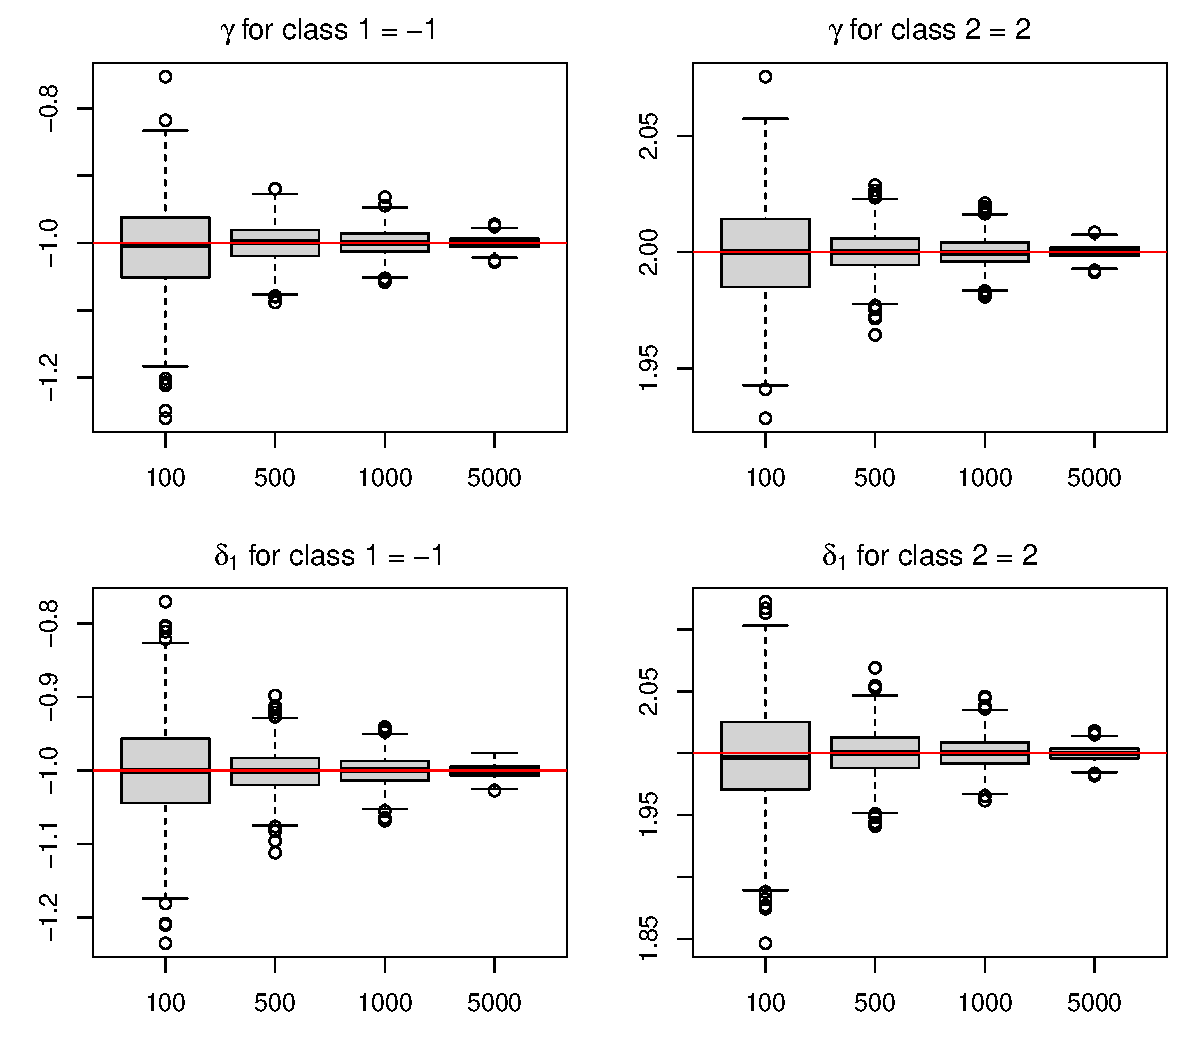
\includegraphics[width =\textwidth]{fig1} 
\end{figure}
\noindent \textsl{Notes: Each figure shows the distribution of the parameters across the 1,000 MC samples. The red horizontal line represents the true value of the parameter.}

\begin{figure}[H]
	\caption{E1: Distribution of $\rho$  and $\pi$ for both classes by sample size}\label{fig:figure2}
	\centering
	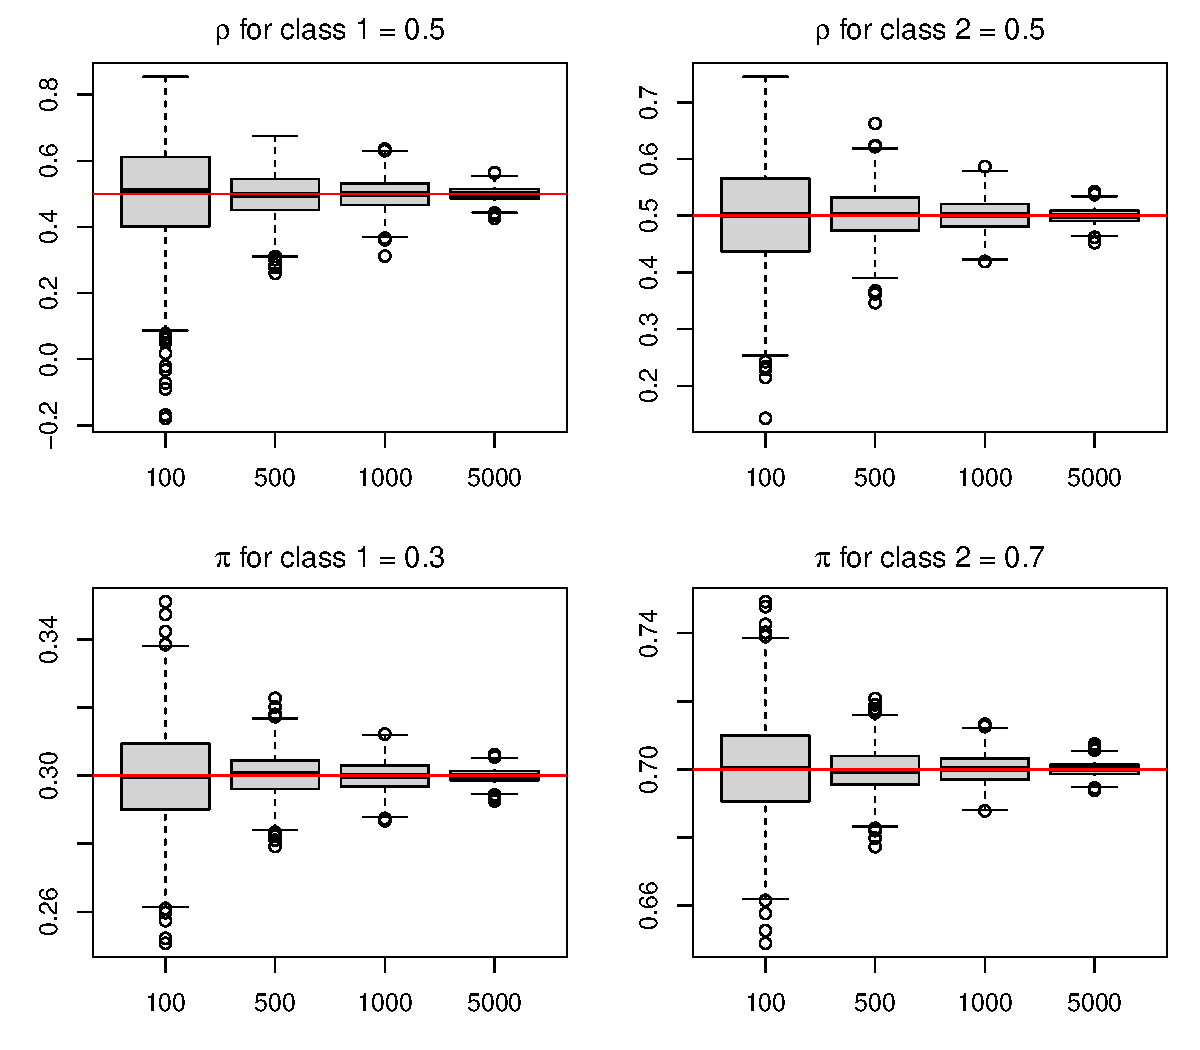
\includegraphics[width =\textwidth]{fig2} 
\end{figure}
\noindent \textsl{Notes: Each figure shows the distribution of the parameters across the 1,000 MC samples. The red horizontal line represents the true value of the parameter.}


\pagebreak
%------------------------------
\section*{Tables}
%------------------------------

\begin{longtable}{lcccccccc}
	\caption{True values of the parameters for MC experiments}\label{tab:experiments} \\
		\midrule
		 \multicolumn{9}{l}{\textbf{E1}: \emph{Endogeneity and power in both classes}} \\
		\midrule
		& $\beta_0$  & $\gamma$ & $\delta_0$  & $\delta_1$ & $\rho$ & $\sigma_{\epsilon}$ & $\sigma_{\upsilon}$ & $\pi$ \\
		\midrule
		Class 1 & -1 & -1  & -1  &  -1 & 0.5 & 1 & 1 & 0.3\\
		Class 2 &  1 &  2  &  1  &  2  & 0.5 & 1 & 1 & 0.7\\
		\midrule
	   \multicolumn{9}{l}{\textbf{E2}: \emph{Endogeneity, but no power in class 1}} \\
	   \midrule
	   & $\beta_0$  & $\gamma$ & $\delta_0$  & $\delta_1$ & $\rho$ & $\sigma_{\epsilon}$ & $\sigma_{\upsilon}$ & $\pi$ \\
	   \midrule
	   Class 1 & -1 & -1  & -1  &  0 & 0.5 & 1 & 1 & 0.3\\
	   Class 2 &  1 &  2  &  1  &  2  & 0.5 & 1 & 1 & 0.7\\
	   \midrule
\end{longtable}
\noindent \textsl{Notes: Value of the true parameters in each class and experiment.}


\begin{longtable}{lcccccccc}
	\caption{E1: Simulation results for LCIV parameters\label{tab:table1}} \\ 
	\toprule & \multicolumn{2}{c}{$N$ = 100} & \multicolumn{2}{c}{$N$ = 500} & \multicolumn{2}{c}{$N$ = 1000} &  \multicolumn{2}{c}{$N$ = 5000} \\
	\toprule
	& Bias & RMSE & Bias & RMSE & Bias & RMSE & Bias & RMSE \\ 
	\midrule
	$\gamma_{1}$ & -0.0048 & 0.0657 & -0.0003 & 0.0281 & 0.0004 & 0.0197 & 0.0001 & 0.0085 \\ 
	$\gamma_{2}$ & -0.0001 & 0.0206 & 0.0000 & 0.0089 & -0.0001 & 0.0063 & 0.0001 & 0.0028 \\ 
	$\delta_{11}$ & 0.0012 & 0.0671 & -0.0008 & 0.0277 & 0.0000 & 0.0200 & -0.0007 & 0.0090 \\ 
	$\delta_{12}$ & -0.0023 & 0.0414 & 0.0003 & 0.0183 & 0.0001 & 0.0129 & -0.0003 & 0.0056 \\ 
	$\rho_{1}$ & -0.0026 & 0.1577 & -0.0033 & 0.0718 & -0.0014 & 0.0491 & -0.0011 & 0.0215 \\ 
	$\rho_{2}$ & -0.0017 & 0.0933 & 0.0016 & 0.0421 & 0.0003 & 0.0282 & -0.0002 & 0.0134 \\ 
	$\pi_{1}$ & -0.0004 & 0.0144 & 0.0003 & 0.0063 & -0.0002 & 0.0044 & -0.0000 & 0.0021 \\ 
	$\pi_{2}$ & 0.0004 & 0.0144 & -0.0003 & 0.0063 & 0.0002 & 0.0044 & 0.0000 & 0.0021 \\ 
	\bottomrule
\end{longtable}
\noindent \textsl{Notes: Results for experiment 2. The number of MC samples is $S=1000$. The bias for each parameter $\theta_k$ is computed as $(1/S)\sum_{s = 1}^S(\widehat{\theta}_{ks} - \theta_{0k})$, where $\theta_{0k}$ is the true value of the parameter. The Means Squared Error is computed as $\textrm{Bias}_k^2 + \var(\widehat{\theta}_k)$, where $\var(\widehat{\theta}_k)$ is the variance of the estimates across the MC samples.}

\newpage
\begin{longtable}{lcccccccc}
	\caption{E1: Simulation results for causal parameters}\label{tab:table2} \\ 
	\toprule & \multicolumn{2}{c}{$N$ = 100} & \multicolumn{2}{c}{$N$ = 500} & \multicolumn{2}{c}{$N$ = 1000} &  \multicolumn{2}{c}{$N$ = 5000} \\
	\toprule
	& Mean & SD & Mean & SD & Mean & SD & Mean & SD \\ 
	\midrule
	ATE & 1.0998 & 0.0499 & 1.0992 & 0.0221 & 1.1005 & 0.0150 & 1.1002 & 0.0072 \\ 
	ATEM & 1.0986 & 0.0589 & 1.0996 & 0.0223 & 1.1003 & 0.0147 & 1.1001 & 0.0073 \\ 
	IV & 2.8966 & 0.4008 & 2.8252 & 0.1487 & 2.8252 & 0.1070 & 2.8213 & 0.0465 \\ 
	\bottomrule
\end{longtable}
\noindent \textsl{Notes: ATE is the average treatment effect computed for the well-specified model, ($Q = 2$). ATEM is the ATE for computed for the miss-specified model, $(Q = 3)$. In both cases, ATE are computed using Equation \eqref{eq:ATE-hat}. The mean and standard deviation are computed for the $S = 1,000$ MC samples. }


\begin{longtable}{lcccccccc}
	\caption{E2: Simulation results for LCIV parameters\label{tab:table3}} \\ 
	\toprule & \multicolumn{2}{c}{$N$ = 100} & \multicolumn{2}{c}{$N$ = 500} & \multicolumn{2}{c}{$N$ = 1000} &  \multicolumn{2}{c}{$N$ = 5000} \\
	\toprule
	& Bias & RMSE & Bias & RMSE & Bias & RMSE & Bias & RMSE \\ 
	\midrule
	$\gamma_{1}$ & 0.6626 & 9.9453 & 0.3207 & 8.2491 & 0.4009 & 6.9113 & 0.8328 & 5.6113 \\ 
	$\gamma_{2}$ & 0.0010 & 0.0206 & 0.0006 & 0.0088 & 0.0006 & 0.0065 & 0.0004 & 0.0032 \\ 
	$\delta_{11}$ & 0.0004 & 0.0674 & 0.0001 & 0.0270 & 0.0004 & 0.0193 & 0.0005 & 0.0085 \\ 
	$\delta_{12}$ & 0.0037 & 0.0407 & 0.0006 & 0.0180 & 0.0006 & 0.0131 & 0.0005 & 0.0059 \\ 
	$\rho_{1}$ & -0.5119 & 0.8873 & -0.4634 & 0.8537 & -0.4579 & 0.8507 & -0.5182 & 0.8924 \\ 
	$\rho_{2}$ & -0.0208 & 0.1162 & -0.0125 & 0.0660 & -0.0127 & 0.0597 & -0.0145 & 0.0583 \\ 
	$\pi_{1}$ & 0.0003 & 0.0193 & -0.0002 & 0.0086 & -0.0001 & 0.0064 & 0.0001 & 0.0052 \\ 
	$\pi_{2}$ & -0.0003 & 0.0193 & 0.0002 & 0.0086 & 0.0001 & 0.0064 & -0.0001 & 0.0052 \\ 
	\bottomrule
\end{longtable}
\noindent \textsl{Notes: Results for experiment 2. The number of MC samples is $S=1000$. The bias for each parameter $\theta_k$ is computed as $(1/S)\sum_{s = 1}^S(\widehat{\theta}_{ks} - \theta_{0k})$, where $\theta_{0k}$ is the true value of the parameter. The Means Squared Error is computed as $\textrm{Bias}_k^2 + \var(\widehat{\theta}_k)$, where $\var(\widehat{\theta}_k)$ is the variance of the estimates across the MC samples.}

\newpage
\begin{longtable}{lcccccccc}
	\caption{E2: Simulation results for causal parameters \label{tab:table4}} \\ 
	\toprule & \multicolumn{2}{c}{$N$ = 100} & \multicolumn{2}{c}{$N$ = 500} & \multicolumn{2}{c}{$N$ = 1000} &  \multicolumn{2}{c}{$N$ = 5000} \\
	\toprule
	& Mean & SD & Mean & SD & Mean & SD & Mean & SD \\ 
	\midrule
	ATE & 1.2961 & 2.9173 & 1.1983 & 2.4607 & 1.2203 & 2.0548 & 1.3516 & 1.6582 \\ 
	ATEM & 1.2495 & 2.6833 & 1.1821 & 2.5962 & 1.1729 & 2.0715 & 1.2541 & 1.5848 \\ 
	IV & 2.0000 & 0.0451 & 2.0001 & 0.0187 & 2.0002 & 0.0133 & 1.9999 & 0.0059 \\ 
	\bottomrule
\end{longtable}
\noindent \textsl{Notes: ATE is the average treatment effect computed for the well-specified model, ($Q = 2$). ATEM is the ATE for computed for the miss-specified model, $(Q = 3)$. In both cases, ATE are computed using Equation \eqref{eq:ATE-hat}. The mean and standard deviation are computed for the $S = 1,000$ MC samples. }

%%%%%%%%%%%%%%%
% Appendices %
%%%%%%%%%%%%%%%

\pagebreak
\newpage
\appendix
\numberwithin{table}{section}
\numberwithin{figure}{section}
\numberwithin{equation}{section}

%----------------------------------------------------------------------------------
\section{Additional Figures}\label{app:add-tables}
%----------------------------------------------------------------------------------

\begin{figure}[H]
	\caption{E1: Distribution of causal parameters by sample size}\label{fig:figure-A1}
	\centering
	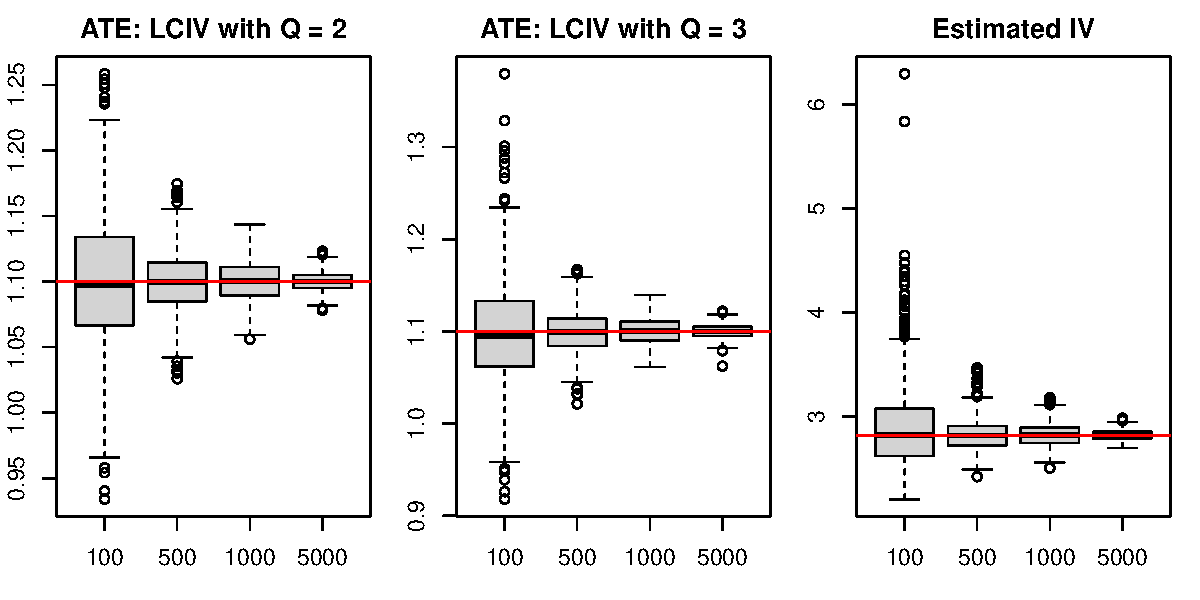
\includegraphics[width =\textwidth]{fig3a-1} 
\end{figure}


\begin{figure}[H]
	\caption{E2: Distribution of $\gamma$ and $\delta_1$ for both classes by sample size}\label{fig:figure-A2}
	\centering
	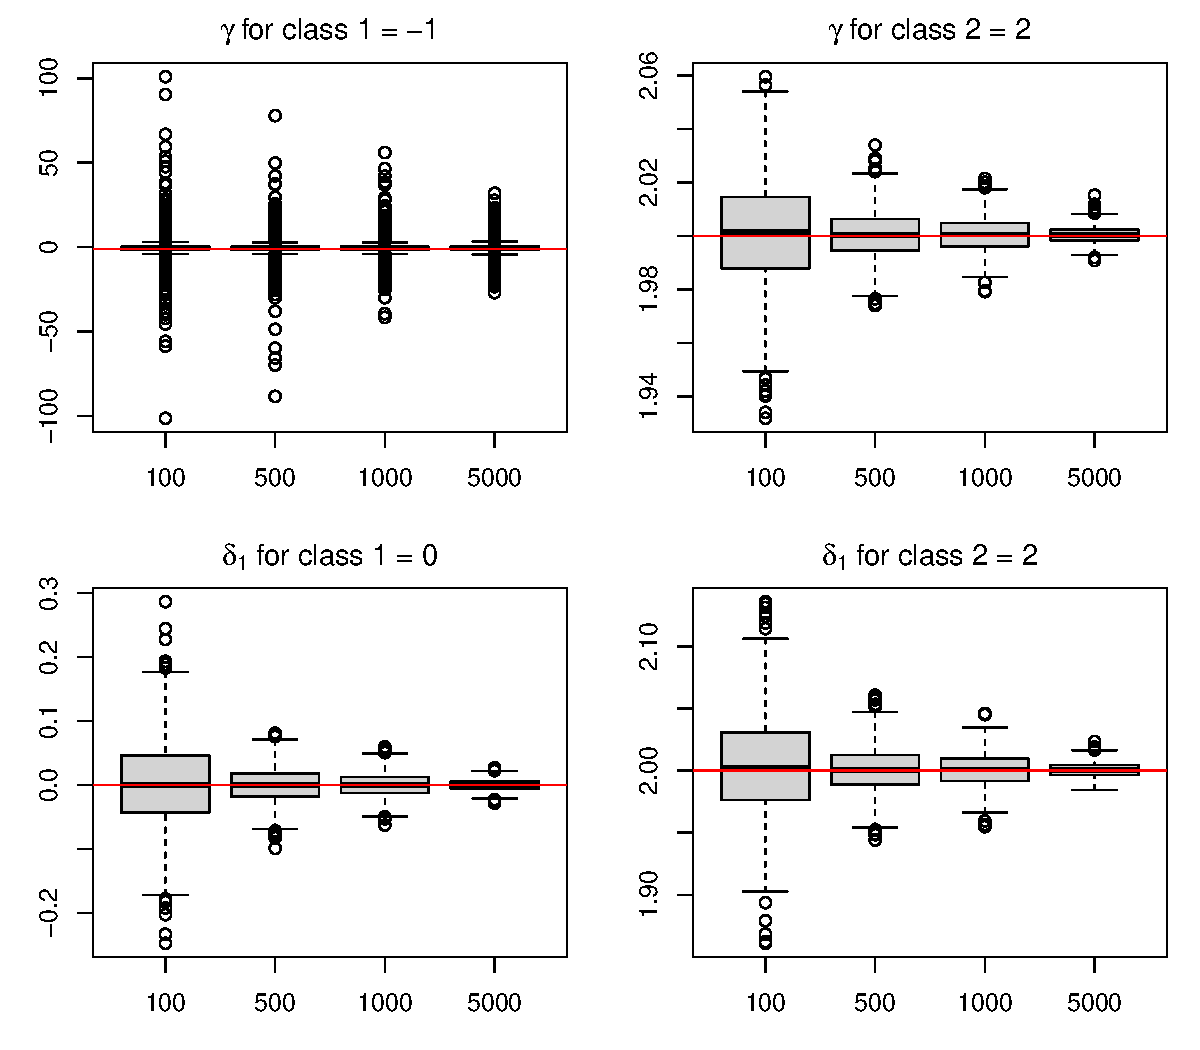
\includegraphics[width =\textwidth]{fig1c-1} 
\end{figure}

\begin{figure}[H]
	\caption{E2: Distribution of $\rho$  and $\pi$ for both classes by sample size}\label{fig:figure-A3}
	\centering
	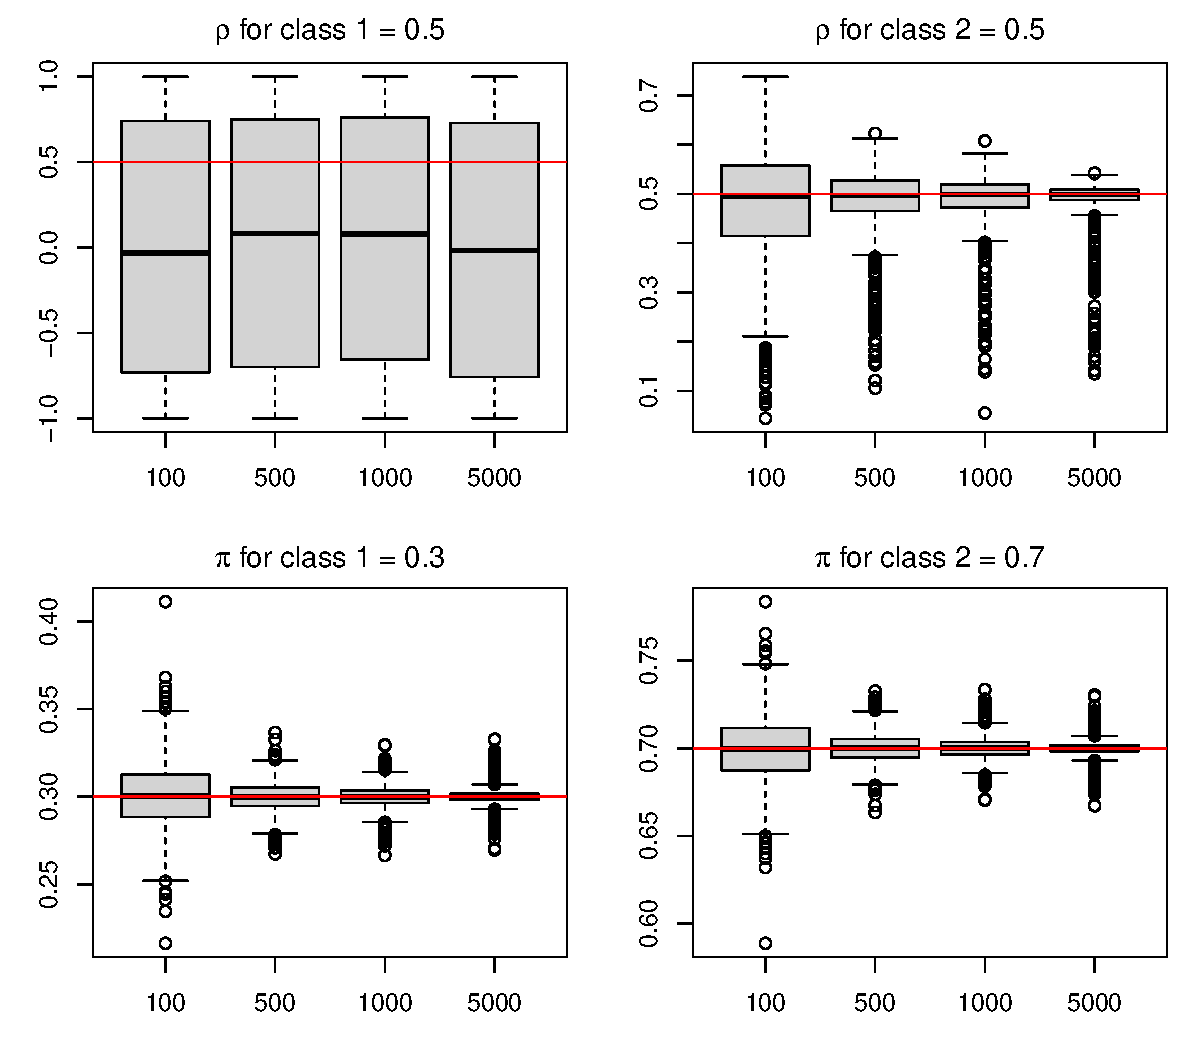
\includegraphics[width =\textwidth]{fig2c-1} 
\end{figure}

\begin{figure}[H]
	\caption{E2: Distribution of causal parameters by sample size}\label{fig:figure-A4}
	\centering
	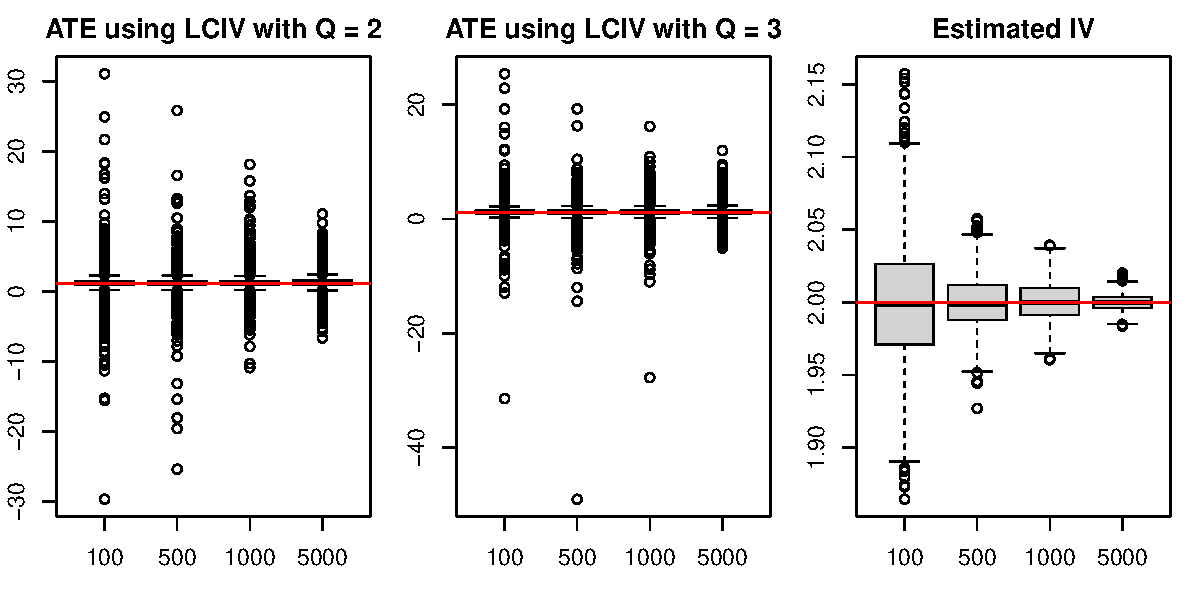
\includegraphics[width =\textwidth]{fig3c-1} 
\end{figure}




%----------------------------------------------------------------------------------
\section{Appendix: IV estimator under treatment and instrument heterogeneity}\label{app:iv-het}
%----------------------------------------------------------------------------------

For simplicity, assume a model with continuous heterogeneity:
\begin{equation}\label{eq:simple-model-cont}
	\begin{aligned}
		y_{1i}   & =  \beta_{0i}  + \gamma_{i}y_{2i}  + \epsilon_{i}, \\
		y_{2i}   & =  \delta_{0i} + \delta_{1i} z_{i} + \upsilon_{i}.
	\end{aligned}
\end{equation}

It is well known that the IV estimator will converge to
\begin{equation}\label{eq:IV-derivation}
	\widehat{\gamma}_{\textrm{IV}} \pto \frac{\cov(y_{1i}, z_{i})}{\cov(y_{2i}, z_i)}. 
\end{equation}

Thus, using the model in Equation \eqref{eq:simple-model-cont} and assuming that the random parameters are distributed independently of $\epsilon_i$, $\upsilon_i$, and $z_i$, the denominator of \eqref{eq:IV-derivation} is expressed as
\begin{equation}
	\begin{aligned}
			\cov(y_{2i}, z_{i}) & = \cov(\delta_{0i} + \delta_{1i} z_{i} + \upsilon_{i}, z_i), \\
			                    & = \cov(\delta_{0i}, z_i) + \cov(\delta_{1i}z_i, z_{i})+ \cov(\upsilon_{i}, z_i),\\
			                    & = \cov(\delta_{1i}z_i, z_{i}),\\
			                    & = \E(\delta_{1i})\var(z_i),
	\end{aligned}	
\end{equation}
%
where the third equality follows because $\cov(\upsilon_i, z_i) = 0$ by assumption, and because $\cov(\delta_{0i}, z_i) = \E\left[\left(z_i - \E(z_i)\right)\delta_{0i}\right] = \E\lbrace \E\left[\left(z_i - \E(z_i)\right)\delta_{0i}\right]|z_i\rbrace = \E\left[\left(z_i - \E(z_i)\right)\E(\delta_{0i}|z_i)\right] = \E\left(z_i - \E(z_i)\right)\E(\delta_{0i}) = 0$ by law of iterated expectations. The last equality follows because $\cov(\delta_{1i}z_i, z_{i}) = \E\left[\left(z_i - \E(z_i)\right)\delta_{1i}z_i\right] = \E\lbrace \E\left[\left(z_i - \E(z_i)\right)\delta_{1i}z_i\right]|z_i\rbrace = \E\left[\left(z_i - \E(z_i)\right)z_i\right] \E(\delta_{1i})$.

Similarly, for the numerator of \eqref{eq:IV-derivation} we obtain
\begin{equation}
	\begin{aligned}
		\cov(y_{1i}, z_i)  & = \cov(\beta_{0i}  + \gamma_{i}y_{2i} + \epsilon_{i}, z_i), \\
		                   & = \cov(\beta_{0i},z_i) + \cov(\gamma_{i}y_{2i}, z_{i})+ \cov(\epsilon_{i}, z_i), \\
		                   & = \cov(\gamma_i\delta_{1i} z_{i}, z_i), \\
		                   & = \E(\gamma_i\delta_{1i})\var(z_i).
	\end{aligned}
\end{equation}

Then, $\widehat{\gamma}_{\textrm{IV}} \pto \frac{\cov(y_{1i}, z_{i})}{\cov(y_{2i}, z_i)} = \frac{\E(\gamma_i\delta_{1i})}{\E(\delta_{1i})}$. Since in our setup the parameters are distributed assuming a discrete distribution, then
\begin{equation}
		\widehat{\gamma}_{\textrm{IV}} \pto \frac{\E(\gamma_i\delta_{1i})}{\E(\delta_{1i})}= \frac{\sum_{q = 1}^Q\pi_q\gamma_q\delta_{1q}}{\sum_{q = 1}^Q\pi_q\delta_{1q}}.
\end{equation}


%----------------------------------------------------------------------------------
\section{Appendix: Parameter transformation}\label{app:transformation}
%----------------------------------------------------------------------------------

During the optimization procedure of the log-likelihood function the parameters $\sigma_{\epsilon, q}$, $\sigma_{\upsilon, q}$, and $\rho_q$ $\forall q = 1, ..., Q$,  might tend to the boundary points of the parameter space generating identifiability problems of the MLE. To avoid this issue, we make some re-parametrization of the parameters. First, to ensure $\sigma_{\epsilon, q} > 0$ and $\sigma_{\upsilon, q} > 0$, we rather estimate $\ln \nu_{\epsilon, q}$ and $\ln \nu_{\upsilon, q}$  such that
\begin{equation}\label{eq:repsigma}
	\begin{aligned}
	\sigma_{\upsilon, q} & = \exp(\ln \nu_{\epsilon, q}),  \\
	\sigma_{\epsilon, q} & = \exp(\ln \nu_{\epsilon, q}).  
	\end{aligned}
\end{equation}

Second, we force the correlation to remain in the \((-1, +1)\) interval by using the inverse hyperbolic tangent:
\begin{equation}
	\textrm{atanh}(\rho_q) = \tau_q = \frac{1}{2}\log\left(\frac{1 +  \rho_q}{1 - \rho_q}\right),
\end{equation}
where \(\tau_q\) is unrestricted. Therefore, \(\rho_q\) can be obtained using the inverse of \(\tau_q\):
\begin{equation}
	\tau_q^{-1} = \rho_q = \tanh(\tau_q).
	\label{eq:reprho}
\end{equation}

%----------------------------------------------------------------------------------
\section{Appendix: Score function}\label{app:gradient}
%----------------------------------------------------------------------------------

In this section, we provide the gradient of the log-likelihood function using the transformations presented in Appendix \ref{app:transformation}. 

Given the class $q$ that individual $i$ belongs to, the joint distribution of $(y_{1iq}, y_{2iq})$, conditional on $\vz_{iq}$, is $P_{i|q}= f_q(y_{1iq}|y_{2iq}, \vz_{iq})f_q(y_{2iq}|\vz_{iq})$. Under Assumption \ref{assu:distribution}, we can write $\epsilon_{iq}|\upsilon_{iq} = \left[(\rho_q\sigma_{q, \epsilon})/\sigma_{q, \upsilon}\right]\upsilon_{iq}  + \eta_{iq}$, where $\eta_{iq}\sim\rN\left(0, \left[1 - \rho_{q}^2\right]\sigma_{q, \epsilon}^2\right)$. Then, replacing the error term into Equation \eqref{eq:first_eqLC} yields:
\begin{equation*}
	y_{1iq}|y_{2iq} =  \vx_{iq}^\top\vbeta_q + \left[(\rho_q\sigma_{q, \epsilon})/\sigma_{q, \upsilon}\right]\upsilon_{iq}   + \eta_{iq}.
\end{equation*}

Since $\upsilon_{iq} = y_{2iq} - \vz_{iq}^\top\vdelta_q$, then the probability of individual $i$ conditional on $y_{2iq}$ and $\vz_{iq}$ is
\begin{equation}\label{eq:conditional}
	\begin{aligned}
		f_q(y_{1iq}|y_{2iq}, \vz_{iq}) & = \rN\left(\vx_{iq}^\top\vbeta_q + \frac{\sigma_{q, \epsilon}}{\sigma_{q, \upsilon}}\rho_q(y_{2iq}-\vz_{iq}^\top\vdelta_q), (1 - \rho^2_q)\sigma_{q, \epsilon}^2\right), \\
		& = \frac{1}{\sqrt{\left(1 - \rho_{q}^2\right)\sigma_{q, \epsilon}^2}}\phi\left(\frac{y_{1iq}-\vx_{iq}^\top\vbeta_q - \frac{\sigma_{q, \epsilon}}{\sigma_{q, \upsilon}}\rho_q(y_{2iq}-\vz_{iq}^\top\vdelta_q)}{\sqrt{(1 - \rho^2_q)\sigma_{q, \epsilon}^2}}\right),
	\end{aligned}
\end{equation}
where $\phi(\cdot)$ is the standard normal density function. 

Since $y_{2i}|\vz_{iq}\sim \rN(\vz_{iq}^\top\vdelta_q, \sigma_{q,\upsilon}^2)$, the conditional (on $q$) marginal distribution is:
\begin{equation}\label{eq:marginal}
	f_q(y_{2iq}|\vz_{iq}) = \frac{1}{\sigma_{q, \upsilon}}\phi\left(\frac{y_{2iq} - \vz_{iq}^\top\vdelta_q}{\sigma_{q, \upsilon}}\right).
\end{equation}

Using Equations \eqref{eq:conditional} and \eqref{eq:marginal}, we obtain Equation \eqref{eq:joint-distribution}.


The contribution of each individual to the log-likelihood function is:
\begin{equation}\label{eq:log-like-app}
	\begin{aligned}
		\ell_i(\vtheta) &  = \ln P_i(\vtheta) = \ln \left[\sum_{q = 1}^Q \pi_{iq}(\vlambda_q)P_{i|q}(\vzeta_q)\right], \\
	\end{aligned}
\end{equation}
%
where $\vtheta = \left(\vzeta_1^\top, \vzeta_2^\top, ..., \vzeta_Q^\top, \vlambda_1^\top, \vlambda_2^\top, ...., \vlambda_Q^\top\right)^\top$,  $\vlambda_1 = \vzeros$ for identification, $\vzeta_q = (\vbeta_q^\top, \vdelta_q^\top, \sigma_{q, \epsilon}, \sigma_{q, \upsilon}, \rho_q)^\top$ is an $\left(K + P + 3\right)$-dimensional vector, and $\vlambda_q$ is an $L$-dimensional vector for $q = 1, ..., Q$. 

Taking the derivative of \eqref{eq:log-like-app} with respect to $\vzeta_q$ yields
\begin{equation}\label{eq:der_zeta_q}
	\begin{aligned}
		\underset{(K + P + 3)\times 1}{\frac{\partial \ell_i(\vtheta)}{\partial \vzeta_q}} & = \left[\frac{1}{\sum_{q = 1}^Q \pi_{iq}P_{i|q}}\right]\left[\pi_{iq}\frac{\partial P_{i|q}}{\partial \vzeta_q}\right], \\
		& = \left[\frac{\pi_{iq}P_{i|q}}{\sum_{q = 1}^Q \pi_{iq}P_{i|q}}\right]\left[\frac{1}{P_{i|q}}\frac{\partial P_{i|q}}{\partial\vzeta_q}\right], \\
		& = \left[w_{iq}\frac{\partial \ln P_{i|q}}{\partial \vzeta_q}\right],\quad q = 1, ..., Q,
	\end{aligned}
\end{equation}
%
where:
\begin{equation*}
	w_{iq} = \frac{\pi_{iq}P_{i|q}}{\sum_{q = 1}^Q \pi_{iq}P_{i|q}}=\frac{\pi_{iq}P_{i|q}}{P_i},
\end{equation*}
%
is a weight so that $0< w_{iq} < 1$ and $\sum_{q = 1}^Qw_{iq} = 1$.

Similarly, taking the derivative of \eqref{eq:log-like-app} with respect to $\vlambda_q$ yields
\begin{equation*}
		\begin{aligned}
		\frac{\partial \ell_i(\vtheta)}{\partial \vlambda_q}  =  \left[\frac{1}{P_i}\sum_{q = 1}^QP_{i|q}\pi_{iq}\frac{\partial \ln \pi_{iq}}{\partial \vlambda_q}\right],
		\end{aligned}
\end{equation*}
%
where $\ln \pi_{iq}= \vh_i^\top\vlambda_q- \ln\left(\sum_{c = 1}^Q\exp\left(\vh_i^\top\vlambda_c\right)\right)$. Thus
\begin{equation*}
	\begin{aligned}
		\frac{\partial \ln \pi_{iq}}{\partial \vlambda_q} = \mathbbm{1}\left(q = c\right)\vh_i - \pi_{iq}\vh_i.
	\end{aligned}
\end{equation*}

To derive $\partial \ln P_{i|j}(\vzeta_q)/ \partial \vzeta_q$ in Equation \eqref{eq:der_zeta_q}, note that the logarithm of Equation \eqref{eq:joint-distribution} is
\begin{equation*}
	\ln P_{i|q} = \ln(1) - \ln\left(\sqrt{(1 - \rho^2_q)\sigma_{q, \epsilon}^2}\right) +\ln \left[\phi(a_{iq})\right] + \ln(1) - \ln(\sigma_{q,\upsilon}) + \ln \left[\phi(b_{iq})\right],
\end{equation*}
%
where we use the following notation and transformations introduced in Appendix \ref{app:transformation}: 
\begin{equation*}
	\begin{aligned}
		P_i & = \sum_{q = 1}^{Q}\left(\pi_{iq} P_{i|q} \right),\\
		P_{i|q} & = \left[\frac{1}{\sqrt{\left(1 - \rho_{q}^2\right)\sigma_{q, \epsilon}^2}}\phi\left(a_{iq}\right)\right]\left[\frac{1}{\sigma_{q, \upsilon}}\phi\left(b_{iq}\right)\right],\\
		a_{iq} & = \frac{y_{1iq}-\vx_{iq}^\top\vbeta_q - \frac{\sigma_{q, \epsilon}}{\sigma_{q, \upsilon}}\rho_q(y_{2iq}-\vz_{iq}^\top\vdelta_q)}{\sqrt{(1 - \rho^2_q)\sigma_{q, \epsilon}^2}},\\
		b_{iq} & = \frac{y_{2iq}-\vz_{iq}^\top\vdelta_{q}}{\sigma_{\upsilon,q}}, \\
		\sigma_{\epsilon,q} & = \exp(\ln \nu_{\epsilon,q}), \\
		\sigma_{\upsilon,q} & = \exp(\ln \nu_{\upsilon,q}), \\
		\rho_q &= \tanh(\tau_q) = \frac{\exp(2\tau_q) - 1}{\exp(2\tau_q) + 1}.\\
	\end{aligned}
\end{equation*}

Using this notation, the derivative $\partial \ln P_{i|q}/\partial \vzeta_q$ is
\begin{equation*}
	\begin{aligned}
		\underset{(K\times 1)}{\frac{\partial \ln P_{i|q}}{\partial \vbeta_q}} & = \left[\frac{\phi'(a_{iq})}{\phi(a_{iq})}\right]\left[\frac{\partial a_{iq}}{\partial \vbeta_q}\right] = - a_{iq}\left[\frac{\partial a_{iq}}{\partial \vbeta_q}\right], \\
		\underset{(P\times 1)}{\frac{\partial \ln P_{i|q}}{\partial \vdelta_q}} & = \left[\frac{\phi'(a_{iq})}{\phi(a_{iq})}\right]\left[\frac{\partial a_{iq}}{\partial \vdelta_q}\right] + \left[\frac{\phi'(b_{iq})}{\phi(b_{iq})}\right]\left[\frac{\partial b_{iq}}{\partial \vdelta_q}\right] = -a_{iq}\left[\frac{\partial a_{iq}}{\partial \vdelta_q}\right]  -b_{iq}\left[\frac{\partial b_{iq}}{\partial \vdelta_q}\right], \\
		\underset{(1\times 1)}{\frac{\partial \ln P_{i|q}}{\partial \ln \nu_{\epsilon, q}}} & = -1 + \left[\frac{\phi'(a_{iq})}{\phi(a_{iq})}\right]\left[\frac{\partial a_{iq}}{\partial \ln \nu_{\epsilon, q}}\right] = -1 - a_{iq}\left[\frac{\partial a_{iq}}{\partial \ln \nu_{\epsilon, q}}\right], \\
	\underset{(1\times 1)}{\frac{\partial \ln P_{i|q}}{\partial \ln \nu_{\upsilon, q}}} & = -1 + \left[\frac{\phi'(a_{iq})}{\phi(a_{iq})}\right]\left[\frac{\partial a_{iq}}{\partial \ln \nu_{\upsilon, q}}\right] + \left[\frac{\phi'(b_{iq})}{\phi(b_{iq})}\right]\left[\frac{\partial b_{iq}}{\partial \ln \nu_{\upsilon, q}}\right], \\
	& = -1 -a_{iq}\left[\frac{\partial a_{iq}}{\partial \ln \nu_{\upsilon, q}}\right] - b_{iq}\left[\frac{\partial b_{iq}}{\partial \ln \nu_{\upsilon, q}}\right],  \\
	   \underset{(1\times 1)}{\frac{\partial \ln P_{i|q}}{\partial \tau_q}} & = \rho_q +  \left[\frac{\phi'(a_{iq})}{\phi(a_{iq})}\right]\left[\frac{\partial a_{iq}}{\partial \tau_q}\right] = \rho_q -a_{iq}\left[\frac{\partial a_{iq}}{\partial \tau_q}\right].
	\end{aligned}
\end{equation*}
%
where we use the fact that $\phi'(z) = -z \phi(z)$ so that $\phi'(z)/\phi(z)= -z$. The derivatives of $a_{iq}$ and $b_{iq}$ are
\begin{equation*}
	\begin{aligned}
		\frac{\partial a_{iq}}{\partial \vbeta_q} & = - \left(\frac{1}{\sqrt{(1 - \rho^2_q)\sigma_{q, \epsilon}^2}}\right)\vx_{iq}, \\  
		\frac{\partial a_{iq}}{\partial \vdelta_q}  & =  \left(\frac{1}{\sqrt{(1 - \rho^2_q)\sigma_{q, \epsilon}^2}}\right)\left(\frac{\sigma_{q, \epsilon}\rho_q}{\sigma_{\upsilon,q}}\right)\vz_{iq}, \\
		\frac{\partial a_{iq}}{\partial \ln \nu_{q, \epsilon}} & = -\frac{\left(y_{1iq}-\vx_{iq}^\top\vbeta\right)}{\sqrt{(1 - \rho^2_q)\sigma_{q, \epsilon}^2}},\\ 
		\frac{\partial a_{iq}}{\partial \ln \nu_{q, \upsilon}} &= \frac{\sigma_{q,\epsilon}\rho_q}{\sqrt{(1 - \rho^2_q)\sigma_{q, \epsilon}^2}}b_{iq}, \\ 
		\frac{\partial a_{iq}}{\partial\tau_{q}}  & = \frac{\left(y_{1iq}-\vx_{iq}^\top\vbeta_q\right)\rho_q- b_{iq}\sigma_{q, \epsilon}}{\sqrt{(1 - \rho^2_q)\sigma_{q, \epsilon}^2}}, \\
		\frac{\partial b_{iq}}{\partial \vdelta_q} & = -\left(\frac{1}{\sigma_{q, \upsilon}}\right)\vz_{iq}, \\ 
		\frac{\partial b_{iq}}{\partial \ln \nu_{q, \upsilon}} & = -b_{iq}, \\
	\end{aligned}
\end{equation*}
%
where $d \tanh(\tau_q) / d \tau_q = \textrm{sech}^2(\tau_q) = 1- \tanh^2(\tau_q)$. 

Finally, the contribution of each individual to the score function for each $q = 1, ..., Q$ is
\begin{equation}
	\vs_{iq}(\vtheta) =\begin{pmatrix}
		               w_{iq}\left[\frac{(y_{1iq}-\vx_{iq}^\top\vbeta_q) - \eta_q(y_{2iq}-\vz_{iq}^\top\vdelta_q)}{(1 - \rho^2_q)\sigma_{q, \epsilon}^2}\right]\vx_{iq} \\
		               w_{iq}\left(-\left[\frac{\left(y_{1iq}-\vx_{iq}^\top\vbeta_q\right) - \eta_q (y_{2iq}-\vz_{iq}^\top\vdelta_q)}{(1 - \rho^2_q)\sigma_{q, \epsilon}^2}\right]\eta_q+\left[\frac{y_{2iq}-\vz_{iq}^\top\vdelta_{q}}{\sigma_{\upsilon,q}^2}\right]\right)\vz_{iq} \\
		               w_{iq}\left(-1 + \left[\frac{\left(y_{1iq}-\vx_{iq}^\top\vbeta\right)^2 - \eta_q(y_{2iq}-\vz_{iq}^\top\vdelta_q)\left(y_{1iq}-\vx_{iq}^\top\vbeta\right)}{(1 - \rho^2_q)\sigma_{q, \epsilon}^2}\right]\right) \\
		               w_{iq}\left[-1 -\left[\frac{(y_{1iq}-\vx_{iq}^\top\vbeta_q)(y_{2qi}-\vz_{iq}^\top\vdelta_q) - \eta_q(y_{2iq}-\vz_{iq}^\top\vdelta_q)^2}{(1 - \rho^2_q)\sigma_{q, \epsilon}^2}\right]\eta_q + \left(\frac{y_{2iq}-\vz_{iq}^\top\vdelta_{q}}{\sigma_{\upsilon,q}}\right)^2\right] \\
		               w_{iq}\left[\rho_q -\left[\frac{(y_{1iq}-\vx_{iq}^\top\vbeta_q) - \eta_q(y_{2iq}-\vz_{iq}^\top\vdelta_q)}{(1 - \rho^2_q)\sigma_{q, \epsilon}^2}\right]\left[\left(y_{1iq}-\vx_{iq}^\top\vbeta_q\right)\rho_q- \left(\frac{y_{2iq}-\vz_{iq}^\top\vdelta_{q}}{\sigma_{\upsilon,q}}\right)\sigma_{q, \epsilon}\right]\right] \\
		              \sum_{c = 1}^Q\frac{P_{i|q}\pi_{ic}}{P_i}\left[\mathbbm{1}\left(q = c\right) - \pi_{ic}\right]\vh_i
	                 \end{pmatrix}
\end{equation}
%
where $\eta_q = (\sigma_{\epsilon, q}/\sigma_{\upsilon, q})\rho_q$. Then $\vs_i(\vtheta)= (\vs_{iq}^\top(\vtheta), ..., \vs_{iQ}^\top(\vtheta))^\top$

\end{document}



